\documentclass{../industrial-development}
\graphicspath{{13-personnel-management-in-it-companies/}}

\title{Управление персоналом в ИТ-компаниях}
\author{Петрова Елена Сергеевна, ПИ-21 МО}
\date{}

\begin{document}

\begin{frame}
  \titlepage
\end{frame}

\section{Обзор задач управления персоналом}

\begin{frame} \frametitle{Понятие управления персоналом}
  \begin{block}{}
     \alert{Управление персоналом} "--- это целенаправленное организованное воздействие на сотрудников компании, с~целью обеспечения эффективного функционирования организации, а также удовлетворения интересов рабочего коллектива
  \end{block}
  
  \begin{itemize}
  \item Субъект (управляющий элемент) "--- рекрутер, HR-менеджер, ИТ-директор, собственники компании, государство
  \item Объект (управляемый элемент) "--- основные компоненты системы управления персоналом: подбор, оценка, обучение и развитие, стимулирование и другие 
    \end{itemize}
\end{frame}

\lecturenotes

\alert{Управление персоналом} "--- это целенаправленное организованное воздействие на сотрудников компании, целью которого является обеспечение наиболее эффективного функционирования организации, а также удовлетворение интересов рабочего коллектива и потребностей отдельно взятого сотрудника~\cite[с.~136]{Bazarov}.

Под \alert{субъектом (управляющим элементом)} понимается совокупность органов и работников, реализующих функции управления персоналом. Субъект управления персоналом "--- тот, от кого зависит качество принятия управленческих решений, а следовательно, последующий результат деятельности работника, подразделения и всей организации в целом; кто обладает функциями управления персоналом. Субъекты  управления персоналом можно разделить на внутренние и внешние. 

Внутренними субъектами управления персоналом являются:
\begin{itemize} 
\item	функциональный аппарат, управляющий процессом подготовки, приема, адаптации, перемещения кадров и т.п.;
\item руководство подчиненными подразделениями и коллективами; 
\item	различные рабочие, профсоюзные и другие общественные организации, выполняющие ряд функций по сплочению коллектива, воспитанию его членов, развитию их творческой активности; 
\item	неформальные лидеры, имеющиеся в коллективе. 
\end{itemize} 

К внешним субъектам деятельности по управлению персоналом относятся:
\begin{itemize} 
\item	государство и те его органы, которые принимают законы, регулирующие сферу трудовых отношений;
\item	профессиональные ассоциации, вырабатывающие рекомендации в области управления;
\item	организации, занимающиеся вопросами труда (в первую очередь, профсоюзы);
\item	собственники компании~\cite[с.~83--84]{Maslova}.
\end{itemize} 

\begin{frame} \frametitle{Основные задачи управления персоналом}
  \begin{enumerate}
  \item Планирование потребности в квалифицированных сотрудниках
  \item Составление штатного расписания и подготовка должностных инструкций
	\item Подбор персонала и формирование коллектива
	\item Анализ и контроль качества работы 
	\item Разработка программ профессиональной подготовки и~повышения квалификации
	\item Аттестация сотрудников: критерии, методики, оценки
	\item Мотивация: заработная плата, премии, льготы, продвижения по службе
	\item Разработка долгосрочного и краткосрочного оперативных планов по работе с персоналом
    \end{enumerate}
\end{frame}

\lecturenotes

Каждой организации присущи определённые цели, которые можно разделить на четыре блока:

\begin{itemize}
\item	экономические;
\item	научно-технические;
\item	производственно-коммерческие;
\item	социальные.
\end{itemize}

\alert{Экономическая цель} "--- получение расчетной модели прибыли от реализации продукции или услуг; \alert{научно-техническая цель} "--- обеспечение заданного научно-технического уровня продукции и разработок, включая повышение производительности труда за счет совершенствования технологии и средств; 
\alert{производственно-коммерческая цель} "--- производство и реализация продукции или услуг в~заданном объеме и с заданной ритмичностью; \alert{социальная цель} "--- достижение заданной степени удовлетворения социальных потребностей работников~\cite[с.~84--85]{Maslova}.

Данные цели достигаются лишь в условиях эффективного управления персоналом организации, создания гибких механизмов управления, позволяющих быстро адаптировать персонал к условиям деятельности компании, сохранить  коллектив и пополнить команду новыми сотрудниками, при~этом обеспечивая как достижение целей организации, так и удовлетворение интересов работников.

\section{Подходы к организации управления персоналом в~ИТ-компании}

\begin{frame} \frametitle{Подходы к организации управления персоналом в ИТ-компании}
 Модели управления персоналом:
    \begin{enumerate}
    \item Управление по целям
    \item Управление посредством мотивации
    \item Рамочное управление
    \end{enumerate}
 Современные концепции и подходы управления персоналом:
    \begin{enumerate}
\item Организационно-административная концепция 
\item Гуманистическая концепция
\item Экономическая концепция
\item Организационно-социальная концепция
\item Компетентностный подход к управлению персоналом
    \end{enumerate}
\end{frame}
\lecturenotes

Эффективность деятельности современных ИТ-компаний в наибольшей степени зависит от того, насколько успешно ими управляют, какие модели и подходы используются при работе с персоналом. Специалисты и исследователи развитых стран выделяют следующие модели и подходы управления персоналом, которые представлены на слайде, далее мы подробнее разберем каждый из них.
	
\begin{frame} \frametitle{Модели управления персоналом}
 \alert{Управление по целям} "--- техника управления, при которой руководство компании и её сотрудники разделяют внутренние цели и понимают, что они означают для~организации
  \begin{itemize}
	\item В начале определенного периода времени устанавливаются цели, от достижения которых может зависеть переменная часть зарплаты сотрудников
\item Регулярно проводится оценка результатов деятельности (performance review), во время которой оценивается достигнутое и ставятся следующие цели
  \end{itemize}
\end{frame}
\lecturenotes

Система \alert{управления по целям} получила широкое признание среди руководителей и менеджеров-практиков, так как она обеспечивает хорошие результаты по достижению запланированных показателей и способствует эффективной совместной деятельности аппарата управления организации.

Принципы управления по целям формулируются исходя из следующих предпосылок:
 \begin{itemize}
\item система управления должна обеспечивать достижение всех целей и задач организации;
\item каждый руководитель, от высшего до первого уровня, должен иметь четкие цели в рамках возложенных на него обязанностей;
\item цели и задачи всех менеджеров согласуются, и в соответствии с этим организуется работа по их выполнению;
\item менеджеры и исполнители совместно формируют функции и добиваются их выполнения путем взаимных консультаций; в идеальном случае формируется иерархия целей, конкретизируемых на каждом последующем уровне при движении сверху вниз.
 \end{itemize}

Процесс управления по целям состоит из четырех этапов:
 \begin{itemize}
\item на первом уточняется круг полномочий и обязанностей руководителей всех уровней;
\item на втором разрабатываются и согласовываются цели и задачи управления в рамках установленных полномочий и обязанностей;
\item на третьем составляются реальные планы достижения поставленных целей;
\item на четвертом производятся контроль, измерение, оценка работы и достигнутых каждым руководителем результатов. По каналам обратной связи осуществляется корректировка заданий, после чего может потребоваться новое согласование целей.
  \end{itemize}

Таким образом, если целеполагание "--- это начало всякой управленческой деятельности, то её обязательным продолжением является определение видов работ, которые нужны для достижения целей. Менеджеры не только составляют планы, но и организуют их выполнение путем формирования структур, процессов и методов, с помощью которых организуется совместная работа. Важное место в деятельности менеджеров занимает разработка систем показателей, с помощью которых измеряются и оцениваются результаты труда каждого отдельного работника подразделения, службы и организации в целом~\cite{Rumyanceva}. 

\begin{frame} \frametitle{Модели управления персоналом}
 \alert{Управление посредством мотивации} "--- техника управления, при которой изучаются потребности, интересы, личные цели сотрудников, а также учитываются возможности интеграции мотивации с требованиями и~целями организации
	  \begin{itemize}
	\item Кадровая политика компании нацелена на развитие человеческих ресурсов, укрепление морально-психологического климата
		\item Наиболее распространенные мотивационные модели:
		\begin{enumerate}
	\item	Рациональная (ориентация на материальные стимулы)
	\item Самореализации (ориентация на возможности самовыражения,
творчество, признание заслуг, перспективы карьеры и профессионального роста)
\item Сопричастности (ориентация на партнерство, участие в~управлении, делегирование полномочий)
	\end{enumerate}
	\end{itemize}
\end{frame}
\lecturenotes

\alert{Управление посредством мотивации} опирается на изучение потребностей, интересов, настроений, личных целей сотрудников, а также на возможность интеграции мотивации с целями компании. Кадровая политика при такой модели ориентируется на развитие человеческих ресурсов, укрепление морально-психологического климата, реализацию социальных программ. В~управленческой науке разработаны различные мотивационные модели, которые нашли широкое применение в развитых странах.
 
Приведем наиболее традиционные:
	  \begin{itemize}
\item рациональная мотивационная модель, в основе которой лежит использование материальных стимулов для награждения или взыскания по результатам работы;
\item мотивационная модель самореализации, суть которой состоит в активизации внутренних мотивов человека: возможности самовыражения, творчества в труде, признания заслуг, расширения самостоятельности и ответственности, перспективах карьеры и профессионального роста;
\item мотивационная модель сопричастности (соучастия) путем сотрудничества, партнерства, участия в управлении, собственности, делегирование полномочий.
	\end{itemize}
Если в развитых странах сегодня на первый план выдвигается мотивационная модель самореализации, то в российских организациях доминирует рациональная мотивационная модель~\cite{Porshnev}. 

\begin{frame} \frametitle{Модели управления персоналом}
\alert{Рамочное управление} "--- техника руководства, при которой
сотрудники могут самостоятельно принимать решения в~пределах заранее установленных границ (рамок)
    \begin{itemize}
	\item Рамки могут задаваться важностью процесса, его непредсказуемостью, нормами
	\item Помогает снять с руководителя решение рутинных задач, разгрузить его для решения задач более высокого уровня
\item Способствует созданию условий для развития инициативы, ответственности и самостоятельности сотрудников, росту удовлетворенности трудом и развивает корпоративный стиль руководства 
     \end{itemize}
		\end{frame}

\lecturenotes

При рамочном управлении исходят из того, что сотрудники могут самостоятельно принимать решения в пределах заранее установленных границ (рамок), которые определяются важностью процесса, его непредсказуемостью, нормами, которые нельзя нарушать.
 
Технология рамочного управления предполагает определение задания, передачу его сотрудникам, создание надлежащей информационной системы, определение границ самостоятельности и способов вмешательства руководителя. Рамочное управление создает условия для развития инициативы, ответственности и самостоятельности работников, повышает уровень организованности и коммуникаций в организации, способствует росту удовлетворенности трудом, развивает корпоративный стиль руководства~\cite{Porshnev}. 

\begin{frame} \frametitle{Модели управления персоналом}
	\begin{table}[h]
\begin{center}
\begin{tabular}{|p{2,5cm}|p{3,5cm}|p{3,5cm}|}
\hline
\tiny \textbf{Модель управления персоналом}   & \tiny \textbf{Преимущества} & \tiny \textbf{Недостатки} \\
\hline
\tiny Управление по целям & 
\tiny 1. Участие в разработке и согласовании целей оказывает мотивирующее влияние на сотрудников

2. Совершенствование системы контроля и оценки работы каждого подразделения и члена организации
& 
\tiny 1. Длительная, сложная и трудоемкая разработка системы целей 

2. При изменении условий, в которых функционирует организация, следует перестраивать и систему целей \\
\hline
\tiny Управление посредством мотивации & 
\tiny 1. Стимулирование сотрудников на~достижение личных и общих коллективных целей

2. Рост удовлетворенности сотрудников выполненной ими работой

&
\tiny 1. Необходимость в тщательном подборе инструментов, т.к. техника не универсальна и не может применяться одинаково к разным компаниям и персоналу

\\
\hline
\tiny Рамочное управление  & 

\tiny
1. Освобождение руководителя от~рутинных задач

2. Создание для сотрудников возможности действовать самостоятельно в определенных границах

3. Повышение уровня организованности и улучшение коммуникаций
&
\tiny 
1. Распространенность только на~часть проблем руководства

2. Трудности с разграничение сфер ответственности и в решении спорных ситуаций
\\

\hline
 \end{tabular}
  \end{center}
   \end{table}
		\end{frame}

\lecturenotes

В таблице представлены преимущества и недостатки рассмотренных моделей управления персоналом: управление по целям, управление посредством мотивации, рамочное управление.

\begin{frame} \frametitle{Современные концепции управления ИТ-персоналом}
  	 \alert{Организационно-административная концепция} "--- техника руководства, при которой основная цель компании состоит в максимально возможном применении трудовых и личностных качеств её сотрудников
	  \begin{itemize}
	\item Сотрудник играет роль ресурса, с помощью которого компания добивается поставленных целей
	\item Главный тезис концепции "--- контроль над системой полномочий сотрудника, его постепенным ростом и развитием как специалиста, способного занять более высокий пост
	  \end{itemize}
 \end{frame}

\lecturenotes

\alert{Организационно-административная концепция управления сотрудниками}

Основой концепции является осуществление работ организационного характера. В качестве основной цели компания должна поставить перед собой потребность в максимально возможном применении трудовых и личностных качеств сотрудников компании.

В данном случае управление осуществляется таким образом, что человек, находящийся на той или иной должности, воспринимается как закрытая вакансия в имеющемся штатном расписании предприятия, т.е. работник играет роль ресурса, с помощью которого компания добивается поставленных целей. HR-специалист должен отбирать новых работников для компании так, чтобы они соответствовали должности, которую будут занимать в дальнейшем. Речь идет о наличии личностных и профессиональных навыков, без которых новичок просто не сможет справиться с занимаемой должностью. 

В итоге, главным тезисом при использовании данной концепции можно считать контроль над~системой полномочий сотрудника, его ответственностью во всевозможных поведенческих ситуациях, постепенным ростом и развитием сотрудника как специалиста, способного занять более высокий пост и обладающего для этого всеми необходимыми качествами~\cite{Sovrconcept}. 

\begin{frame} \frametitle{Современные концепции управления ИТ-персоналом}
 	 \alert{Гуманистическая концепция} "--- техника руководства, при~которой основная цель компании состоит в~формировании условий, в которых сотрудник сможет реализовать себя внутри компании и не продолжит поиски более интересного места работы 
		  \begin{itemize}
		\item Сотрудник воспринимается не просто как обычный член коллектива, которого можно легко сменить "--- а~как главный субъект организации
		\item Главный тезис концепции "--- самоуправление и возможность стимулирования продуктивной работы с~помощью дополнительных благ на рабочем месте
	  \end{itemize}
\end{frame}

\lecturenotes

\alert{Гуманистическая концепция}

В некоторых случаях её именуют концепцией управления человека. При создании данной методики было использовано большое количество форм работы, применяющихся в японском менеджменте. В этом случае каждый работник воспринимается не просто как обычный член коллектива, которого можно легко сменить "--- речь идет о сотруднике как главном субъекте предприятия.

Главной целью данного принципа, которой должен достичь HR-специалист компании, является формирование таких условий, в которых сотрудник захочет реализовать себя внутри предприятия и не продолжать поиски более интересного места работы. Основной тезис концепции подразумевает, что не человек создан для компании, а наоборот "--- компания создана для нужд человека.

Говоря о современных концепциях управления персоналом, нельзя не отметить гуманистическую, как самую удобную для всех сторон рабочего процесса. Сотрудник в данном случае играет роль весомого участника организационной системы функционирования предприятия, ощущая тем самым собственную важность. В данном случае никто не предъявляет какие-либо серьезные требования к профессиональным качествам нового сотрудника. Работнику предстоит самостоятельно выстраивать внутриорганизационные отношения с коллегами, и в данном случае все будет зависеть от того, насколько он сам будет готов выполнить это условие.

Главным тезисом данной концепции следует считать самоуправление и возможность стимулирования продуктивной работы с помощью дополнительных благ на рабочем месте~\cite{Sovrconcept}. 

\begin{frame} \frametitle{Современные концепции управления ИТ-персоналом}

\alert{Экономическая концепция} "--- техника руководства, при~которой основная цель компании состоит в~максимально возможном использовании потенциала сотрудников
  \begin{itemize}
	\item Сотрудник играет роль типичного фактора производства, обязанного выполнять все необходимые распоряжения руководства
	\item Главный тезис концепции "--- подбор таких специалистов, которых необходимо стимулировать с~помощью финансовых благ
	  \end{itemize}
\end{frame}

\lecturenotes

\alert{Экономическая концепция}

В данном случае главной целью ставится максимально возможное использование потенциала работников. HR-отдел должен контролировать, насколько качественно трудовые навыки сотрудников реализуются в производственном процессе, и помогать персоналу реализовать себя в рамках рабочей деятельности.

Здесь человек играет роль типичного фактора производства, обязанного выполнять все необходимые распоряжения руководства. Специалисты HR должны предъявлять к новым сотрудникам целый ряд требований:
\begin{itemize}
\item ответственность;
\item	наличие технических знаний;
\item	исполнительность;
\item	наличие самодисциплины;
\item	возможность подавлять собственные интересы во благо общего дела.
\end{itemize}

Здесь необходимо подбирать только таких работников, которых необходимо стимулировать с помощью финансовых благ. Концепция будет эффективной в том случае, если предприятие ставит перед собой четкие задачи, намечает план действий и учитывает наличие как внешних, так и внутренних факторов~\cite{Sovrconcept}. 

\begin{frame} \frametitle{Современные концепции управления ИТ-персоналом}
 \alert{Организационно-социальная концепция} "--- техника руководства, при которой основная цель компании состоит в создании максимально благоприятной окружающей среды, способствующей наиболее полному использованию потенциала сотрудников
		  \begin{itemize}
			\item Сотрудник является индивидуальностью, ни одного из~сотрудников невозможно заменить кем-то другим
		\item Главный тезис концепции "---  к новым сотрудникам предъявляется большое количество требований, соответствие должности по большому количеству параметров, а также корпоративным устоям компании
		  \end{itemize}
\end{frame}

\lecturenotes

\alert{Организационно-социальная концепция}

В компании, где используется подобная стратегия, осуществляется качественное управление персоналом. В данном случае потенциал сотрудника необходимо раскрыть полностью, и для этого компания обязана создать идеальные условия, в которых работнику будет комфортно выполнять возложенные на него обязанности.

Работник здесь является индивидуальностью, повторить которую никто в компании не сможет. К~новым сотрудникам предъявляется большое количество требований, главным среди которых является соответствие должности по большому количеству параметров, а также корпоративным устоям организации. 

Организационно-социальная концепция подразумевает, что ни одного из сотрудников невозможно заменить кем-то другим, каждый из них является ценностью для компании и показателем её развития. В данном случае HR-специалисты должны подбирать сотрудников, которые бы по своим личным и профессиональным качествам соответствовали организации. В компаниях, использующих подобную концепцию, часто осуществляется обучение персонала, причем оно иногда является узкоспециализированным, что немаловажно при работе в крупной организации~\cite{Sovrconcept}. 

\begin{frame} \frametitle{Современные концепции управления ИТ-персоналом}
	\alert{Компетентностный подход} "---  техника руководства, при~которой основная цель компании состоит в~обеспечении компетентности кадрового персонала 
 \begin{itemize}
\item Принципы кадровой политики компании: 
	 \begin{enumerate}
	\item кадровая стабильность
	\item эффективное стимулирование
	\item «подстраховка» кадров
	\item обмен знаниями
	\item обучение
	 \end{enumerate}
	\item Главный тезис подхода "--- специалист должен не просто обладать определенным набором знаний и умений, полученных в процессе приобретения квалификации, но использовать его и углублять 
  \end{itemize}
\end{frame}

\lecturenotes

\alert{Компетентностный подход к управлению ИТ-персоналом}

В условиях всеобщей глобализации и повышения уровня конкуренции фактор компетентности кадрового персонала становится ключевым. Наивысшая проблематичность подбора персонала и работы с ним объясняется прежде всего тем, что сфера информационных технологий в настоящее время признана одной из самых динамично развивающихся отраслей мирового рынка.

Понятие компетентного специалиста конкретнее отражает интересы ИТ-предприятия при наборе персонала и управлении им, так как динамичность развития сферы информационных технологий предполагает, что специалист должен не просто обладать определенным набором знаний и умений, полученным им в процессе приобретения квалификации, но и использовать его, углублять и наращивать в темпах, соответствующих росту объема знаний в выбранном им направлении.

К тому же в процессе развития информационных технологий некоторые знания, умения и навыки могут отойти на второй план, а часть из них и вовсе исчезнуть из области деятельности, что предполагает необходимость умения специалиста реагировать на такие изменения и ускоренно адаптироваться к ним.

Компетентность обычно рассматривают как совокупность компетенций, сосредоточенных в одном лице, умеющем их применять в условиях функционирования предприятия, наращивать комплекс знаний и навыков и быстро переучиваться при наличии такой необходимости. 

Был выделен ряд принципов, на которых может быть построена кадровая политика ИТ-предприятия на основе идей компетентностного подхода: кадровая стабильность, эффективное стимулирование, «подстраховка» кадров, обмен знаниями, обучение~\cite{Kasyanov}. 

\section{Специфика управления ИТ-персоналом}

\begin{frame} \frametitle{Факторы, влияющие на управление ИТ-персоналом}
  \begin{itemize}
  \item неразвитость российского рынка труда
  \item утечка ИТ-кадров за рубеж
	\item необходимость постоянных усилий для поддержки квалификации ИТ-специалистов
	\item крайне существенная разница в эффективности труда ИТ-специалистов
	\item невозможность совмещения ИТ-специалистами некоторых ролей и обязанностей
	\item рост объема и сложности задач
	\item преобладание творческого подхода при решении задач

    \end{itemize}
\end{frame}

\lecturenotes

Рассмотрим особенности управления специалистами по информационным технологиям, которые отличают эту группу от других и должны быть учтены. 

Первая особенность "--- \alert{неразвитость российского рынка труда}. Западные подходы и теории строятся на том, что рынок труда перенасыщен специалистами, вследствие чего акцент делается на правильную организацию работы по поиску, отбору, найму и мотивации. В российских условиях очень часто приходится сталкиваться с тем, что ИТ-специалист необходимой квалификации просто отсутствует на рынке труда, или, например, с тем, что часто теоретически невозможно организовать быстрое привлечение к работе требуемого специалиста, поскольку на это может потребоваться время, которым организация не располагает. 

Второй особенностью является \alert{утечка кадров за рубеж}, это определяется большим количеством возможностей на ИТ-рынке. Знание английского языка поднимает стоимость на рынке любого ИТ-специалиста, доводя её до международного уровня. 

Другой особенностью является \alert{невозможность совмещения некоторых ролей и обязанностей}, так как это источник риска. То есть невозможность сотрудником брать дополнительную работу по другой профессии (должности), связанную с выполнением других функциональных обязанностей по сравнению с основной работой, из-за широкого перечня требований к знаниям, навыкам, квалификации, компетенциям в профиле должности, утвержденным в компании. 

Еще одна особенность "--- \alert{необходимость постоянных усилий для поддержки квалификации}. В отличие от многих других специальностей ИТ-персоналу требуется время для ознакомления с новыми продуктами, технологиями, так как за 5 "--- 7 лет в области ИТ происходит большое количество революционных изменений, которые обесценивают предыдущие знания и опыт. Поэтому ИТ-специалистам необходимо регулярное дополнительное образование, изучение публикаций и самообразование. Все это должно являться частью их основных обязанностей независимо от специализации, направления деятельности или занимаемого положения. 

Следующая особенность ИТ-персонала "--- \alert{преобладание творческого подхода при решении задач}; если поставленная задача новая, сложная и требует нестандартного, творческого решения.

Другую особенность ИТ-персонала, которую необходимо учитывать в управлении, можно сформулировать как \alert{крайне существенную разницу в эффективности труда ИТ-специалистов}, в особенности разработчиков. Так, опытный и высококвалифицированный разработчик может выполнить некоторые задачи в 10 "--- 15 раз быстрее обычного. Некоторые менеджеры, например, по обслуживанию пользователей, могут в течение 2 "--- 3 лет налаживать эту работу, в то время как руководитель, который уже приобрел этот опыт (особенно, если он положительный) в другой организации, может все наладить за 2 "--- 3 месяца~\cite[с.~51--52]{Tutunik}.

В ИТ-сфере помимо расширения самого сегмента возрастает и сложность задач, которые приходится решать специалистам~\cite{Bogatova}.

\begin{frame} \frametitle{Особенности управления ИТ-персоналом}
  \begin{itemize}
	\item необходимость в разработке технологии привлечения, удержания и мотивирования сотрудников
	\item осуществление непрерывного обучения и переподготовки, как на рабочем месте, так и вне его
	\item предоставление гибкого рабочего графика для~ИТ-специалистов
	\item координирование коллектива для завершения проектов в строго заданные сроки, обеспечивая соответствующее качество
	\item поддержка создания и востребованности новых идей
	\item индивидуальный подход к сотрудникам
	\item возможна зависимость компании от ключевого ИТ-персонала
    \end{itemize}

\end{frame}
\lecturenotes

На слайде представлен ряд особенностей управления ИТ-персоналом, учет которых позволить эффективно управлять сотрудниками компании, поддерживать на высоком уровне и степень участия каждого её члена, и общий результат.

Всё больше ИТ-компаний уделяют внимание разработке собственной технологии привлечения, удержания и мотивации сотрудников, созданию определенной системы стимулов, которая будет способствовать эффективной работе персонала. Ведь в сфере ИТ можно отметить высокую мобильность и текучесть кадров.

ИТ-профессионалы очень ценят возможность обучения и переподготовки на рабочем месте, так как существующие технологии быстро меняются, а новые постоянно появляются, вместе с тем и растет объем и сложность задач. Данная возможность важна для сохранения набора знаний специалистов на современном уровне. 

Многие ИТ-компании предоставляют сотрудникам гибкий график работы, т.е. распределение их рабочего времени так, что работник по своему усмотрению может выбирать ежедневное начало и окончание трудового дня на основе договоренности с работодателем.

Учитывая психологические особенности ИТ-специалистов и вид их деятельности, руководству компании необходимо поддерживать создание новых идей, творческий подход сотрудников к работе, а так же использовать индивидуальный подход к сотрудникам.

Также следует учитывать возможность зависимости компании от ключевого ИТ-персонала. Эта зависимость проявляется в том, что очень часто на практике в организациях после ряда успешных лет работы появляется специалист или группа специалистов, которые обладают знаниями всех деталей функционирования и организации информационных систем, технологических цепочек, носителями уникального и «сокровенного» знания. Они не спешат делиться знаниями и навыками с другими работниками ИТ и постепенно становятся незаменимыми, «без них все начинает останавливаться»~\cite[с.~51--52]{Tutunik}.

\begin{frame} \frametitle{Особенности ИТ-специалистов}
    
  \begin{itemize}
  \item способность генерировать, объединять, развивать новые идеи
	\item способность выполнять работу с высокими требованиями, работать автономно
	\item способность развиваться, обучаться новому, адаптироваться к изменениям и к требованиям высоких технологий
	\item способность, в зависимости от должности, создавать некий интеллектуальный продукт или организовывать условия для создания и использования созданных продуктов
	\item работа, отличающаяся многозадачностью и интенсивностью, ориентированная на достижение уникальных результатов
	\item доход определяется интеллектуальными ресурсами

    \end{itemize}
\end{frame}
\lecturenotes

К особенностям ИТ-специалистов можно отнести такие характеристики, как:
 \begin{itemize}
	\item	способность генерировать, объединять, развивать новые идеи; 
	\item	способность выполнять работу с высокими требованиями, работать автономно;
	\item способность создавать и транслировать ценные знания от поколения к поколению для повышение конкурентоспособности;
	\item способность развиваться, обучаться новому, адаптироваться к изменениям и к требованиям высоких технологий; 
	\item доход определяется интеллектуальными ресурсами; 
	\item работа, отличающаяся многозадачностью и интенсивностью, ориентированная на достижение уникальных результатов;
	\item удовлетворенность этой группы работников зависит от оплаты, смысла работы, процесса принятия решений, взаимоотношений с высшим руководством, перспектив занятости;
	\item высокоразвитое абстрактное мышление и способность предвосхищать новые перспективы, генерировать новые решения и создавать новые процессы;
	\item гибкий рабочий график;
	\item фриланс, возможность удаленной работы;
	\item способность, в зависимости от должности, создавать некий интеллектуальный продукт или организовывать условия для создания и использования созданных продуктов~\cite[с.~2--3]{Zavyalova}.
 \end{itemize}
		
Работа ИТ-специалистов связана с частыми изменениями, высокой степенью неопределенности и новизны создаваемого продукта. Достижение ими конечной цели возможно только при эффективной работе каждого члена команды~\cite{MotivationIT}.

\begin{frame} \frametitle{Психологические особенности ИТ-специалистов}
  \begin{itemize}
	 \item ставят перед собой высокие цели и неукоснительно их добиваются "--- амбициозны, самодостаточны 
		\item нуждаются в свободе принятия решений "--- самостоятельны, независимы
		\item имеют высокий уровень ответственности и лояльности
		\item предпочитают предсказуемость переменам
	\item зависимы от мнения окружающих "--- им важно иметь авторитет в коллективе
	\item имеют невысокую коммуникабельность
    \end{itemize}

\end{frame}
\lecturenotes

Следует обратить внимание и на психологические особенности персонала в ИТ-компаниях, так как по своему менталитету ИТ-специалисты обычно отличаются от сотрудников других профессий. На основании исследования ИТ-профессионалов зарубежными учеными были выделены следующие черты характера и особенности поведения современного преуспевающего профессионального работника в области ИТ, они представлены на слайде.

В действительности ИТ-специалисты обладают разнообразными личностными и профессиональными качествами. Тем не менее, для персонала ИТ-отрасли характерны некоторые особенности, берущие начало в комплексе профессиональных ценностей и неписанных правил поведения, сложившихся за сравнительно небольшой период существования ИТ-отрасли. Такие ценности и образцы поведения передаются ведущими ИТ-специалистами их преемникам через установки профессиональной деятельности, алгоритмы мышления, отдельные поступки и технологические операции и т.д~\cite{OsobenPoveden}. 

\section{Элементы системы управления персоналом}
\begin{frame} \frametitle{Элементы системы управления персоналом}
  
	\centerline{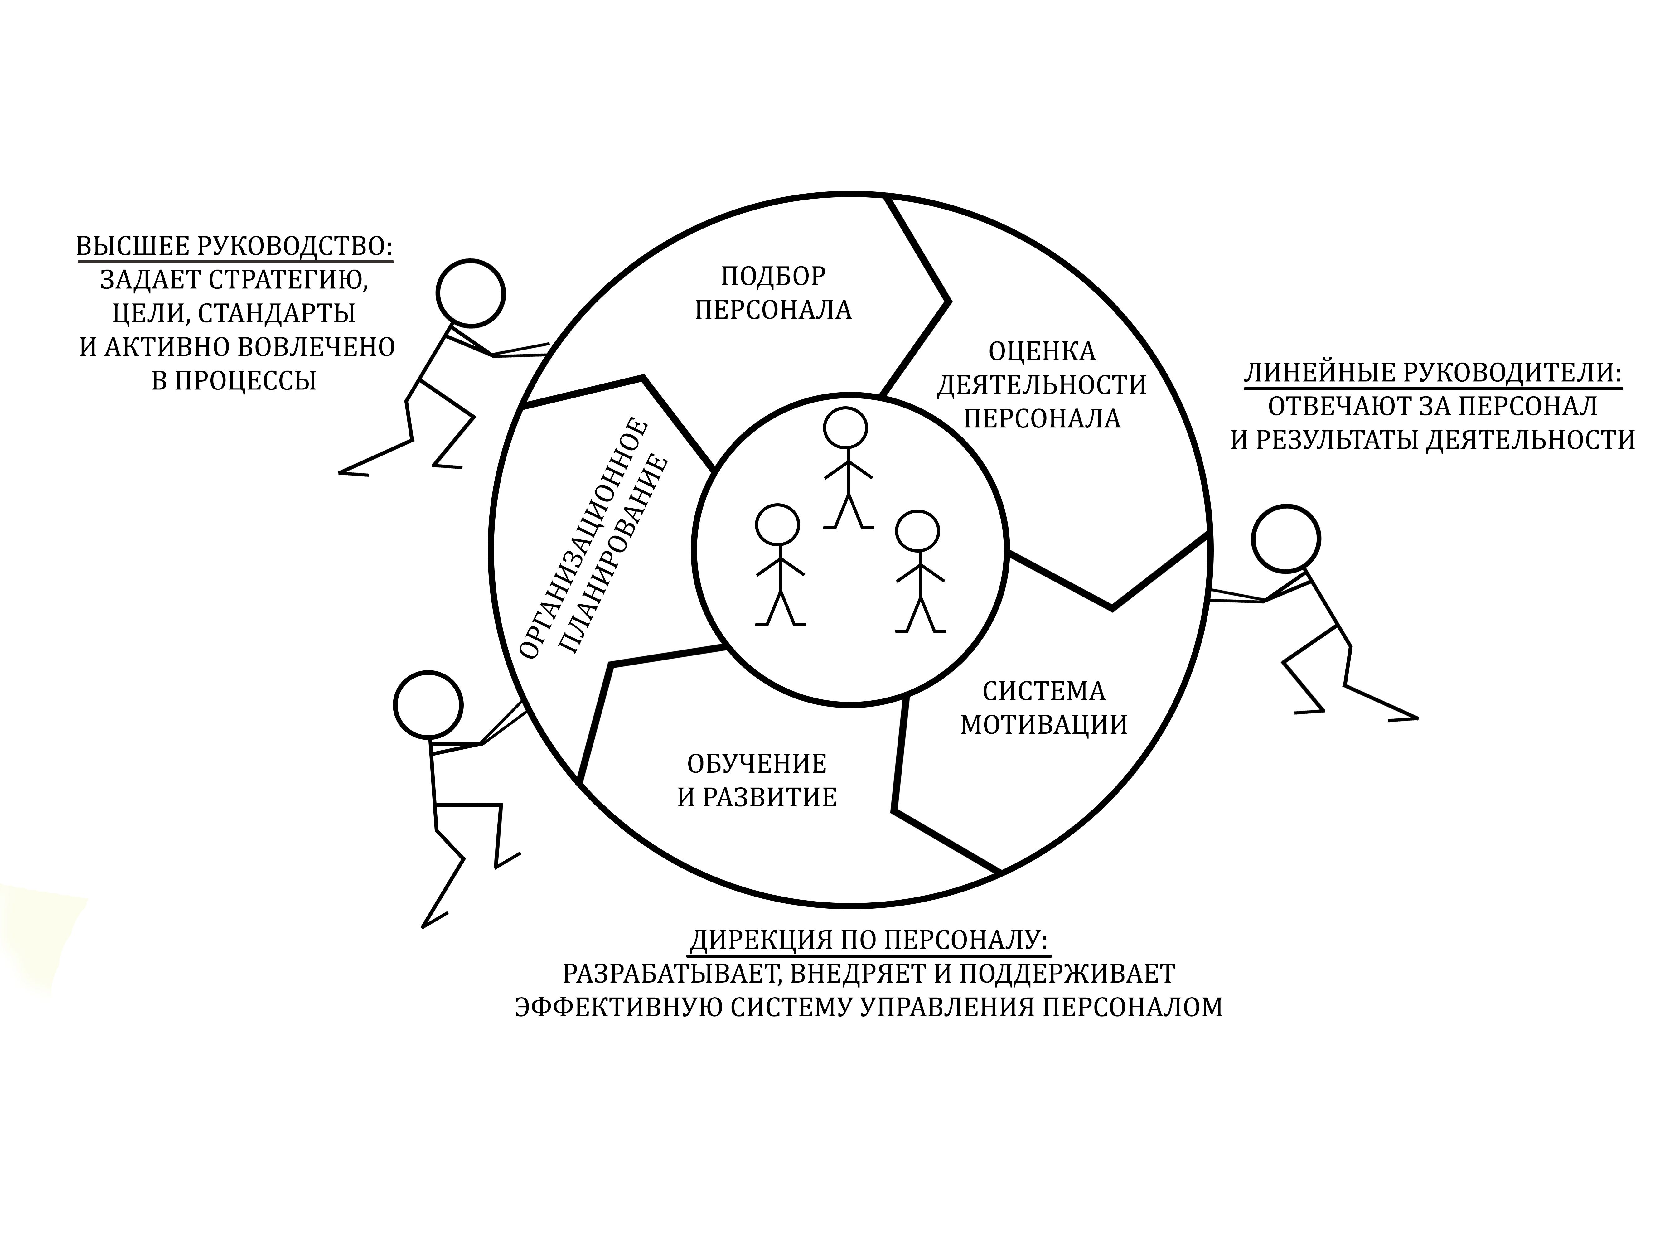
\includegraphics[width=0.9\textwidth]{socpic1.pdf}}
	
\end{frame}

\lecturenotes

Наличие данных составляющих позволяет говорить о том, что в ИТ-компании функционируют базовые элементы управления персоналом. Далее мы рассмотрим каждый элемент системы управления персоналом более подробно.

\begin{frame} \frametitle{Элементы системы управления персоналом}

\begin{itemize}
\item Планирование персонала "--- комплекс мер, направленных на оценку текущих ресурсов, прогнозирование их сокращения, оценку будущей потребности, резервов и способов быстрого замещения специалистов
\item Привлечение персонала "--- комплекс мер, обеспечивающий привлечение требуемых специалистов в заданное время, включая поиск, отбор, наем и первичное развитие персонала
 \end{itemize}
\end{frame}

\lecturenotes

\alert{Планирование персонала} "--- комплекс мер, направленных на оценку текущих ресурсов, прогнозирование их сокращения, оценку будущей потребности в ресурсах, в том числе и в руководящих работниках, оценку резерва персонала и способов быстрого замещения специалистов.

\alert{Привлечение персонала} "--- комплекс мер, обеспечивающий привлечение требуемых специалистов в заданное время. Данные меры включают поиск, вербовку, отбор, наем и первичное развитие персонала.

Наиболее целесообразно начинать построение и развитие системы управления персоналом с планирования ресурсов. Компания должна четко прогнозировать свои будущие потребности в трудовых ресурсах. 

Другая причина актуальности развития системы прогнозирования кроется в текучести кадров. В мировой практике принято заранее готовиться к подобным ситуациям и иметь некоторый резерв специалистов для того, чтобы непредвиденные случаи не привели к остановке работы организации~\cite[с.~52]{Nelarin}.

\begin{frame} \frametitle{Элементы системы управления персоналом}
 \begin{itemize}
 \item Развитие персонала "--- обучение и переподготовка персонала, перемещение, оценка и продвижение персонала, подготовка резервов специалистов и руководителей 	 
				
	\item	Мотивация и стимулирование персонала "--- включают в~себя оплату труда, дополнительные стимуляционные выплаты и систему мотивации труда
			
	\item	Учет персонала "--- комплекс мер по обеспечению кадровой работы в соответствии с требованиями контролирующих органов и потребностями самой компании

 \end{itemize}
\end{frame}

\lecturenotes

\alert{Развитие персонала} "--- включает обучение и переподготовку персонала, перемещение, оценку и продвижение персонала, подготовку резервов специалистов и руководителей.

\alert{Мотивацию и стимулирование персонала} "--- включают оплату труда, дополнительные стимуляционные выплаты и систему мотивации труда.

\alert{Учет персонала} "--- комплекс мер по обеспечению кадровой работы в соответствии с требованиями контролирующих органов и потребностями самой организации. 

Самыми узкими областями в сфере управления персоналом, а потому наименее разработанными, являются развитие персонала, его мотивация, а также учет ресурсов~\cite[с.~52]{Nelarin}.


\subsection{Подбор персонала}

\begin{frame} \frametitle{Подбор персонала}
	Классический пассивный поиск
  \begin{itemize}
	\item Размещение объявлений на сайте компании и на~специализированных ресурсах (hh.ru, superjob.ru и т.п.)
	\item Использование IT job-сервисов (habrahabr.ru, «Мой круг» и djinni.co)
	\item Следует запрашивать у соискателей вместе с резюме примеры их реальных работ (готовых или выполненных по спец. заданию), а у недавних выпускников вузов "--- копию диплома с оценками 
	  \end{itemize}
	
Активный вариант поиска
		  \begin{itemize}
		  \item Работа в социальных сетях, специализированные сервисы (LinkedIn, AmazingHiring), профессиональные форумы разработчиков и «охота за головами» на~профессиональных ИТ-мероприятиях 
		  \end{itemize}
\end{frame}

\lecturenotes

Современный ИТ-рекрутинг (подбор ИТ-персонала) выделяют в отдельную дисциплину, где глубже рассматривается личностный потрет ИТ-специалиста, разбираются ИТ-компетенции и т. д. В качестве отличительной особенности профиля кандидатов выделяют повышенные требования к интеллектуальным способностям и знание широкого перечня технологий, набор которых непрерывно меняется.
 \begin{itemize}
\item	\alert{Классический пассивный поиск} "--- это размещение объявления, желательно креативного содержания. Объявление размещается на сайте компании и на специализированных ресурсах (hh.ru, superjob.ru и т. п.). 

Требования должны быть описаны доступным и понятным языком, обязательно следует указать преимущества работы в вашей компании, соответствующие мотивирующим факторам. Дополнительно советую запрашивать у соискателей вместе с резюме примеры их реальных работ (готовых или выполненных по вашему заданию), а у недавних выпускников вузов "--- копию диплома с оценками. 

\item	\alert{Активный вариант поиска} "--- это работа в социальных сетях, специализированные сервисы (Linked In, Amazing Hiring), профессиональные форумы разработчиков и «охота за головами» на профессиональных ИТ-мероприятиях. Хороших кандидатов можно найти по рекомендации собственных сотрудников, среди работников конкурирующей компании, клиентов, поставщиков и т.п~\cite[с.~274--277]{Pererva}.
  \end{itemize}

\begin{frame} \frametitle{Профиль должности}

\alert{Профиль должности} "--- документ, включающий перечень требований к знаниям, навыкам, квалификации, компетенциям  кандидата, необходимым для успешного выполнения должностных обязанностей
  \begin{itemize}
		\item[1.] Определение профиля должности
  \begin{itemize}
	\item Важно установить уровень развития требуемого специалиста по шкале профессионализма от младшего инженера до руководителя группы
	
	  \end{itemize}
		
		\item[2.] Определение перечня профессиональных компетенций
		  \begin{itemize}
		\item Источник информации "--- база профессиональных стандартов, представленная на сайте Минтруда России
		\item В стандарты заложены градации профессионализма и требования к уровню образования и стажу работы
		  \end{itemize}
  \end{itemize}
\end{frame}

\lecturenotes

\alert{Шаг 1. Определяем должностной уровень}

Важно определить уровень развития требуемого специалиста, то есть того, кто вам нужен именно сейчас, по шкале профессионализма от младшего инженера до руководителя группы. Хороший вариант ранжирования профессиональных навыков принят в e-CF, где профессионализм определяется тремя составляющими: сложностью, самостоятельностью и ответственностью. Именно эти три составляющие вы и должны раскрыть в контексте своей производственной деятельности.

\alert{Шаг 2. Определяем перечень профессиональных компетенций}

Вам необходимо определить исчерпывающий перечень требуемых компетенций с учетом должностного уровня, определенного на первом шаге. Источник информации — база профессиональных стандартов, представленная на сайте Минтруда России (http://profstandart.rosmintrud.ru/). В структуру каждого из стандартов заложены градации профессионализма и требования к уровню образования и стажу работы~\cite[с.~280]{Pererva}.


%%%%%%%%%%%%%%%%%%%%%%%%%%%%%%%%%%%%%%%%%%%%%%

\begin{frame} \frametitle{Пример перечня профессиональных компетенций}
	\begin{table}[h]
\begin{center}
\begin{tabular}{|p{0,5cm}|p{5cm}|p{3,5cm}|}
\hline
\tiny \textbf{Код}   & \tiny \textbf{Вид профессиональной деятельности} & \tiny \textbf{Профессиональный стандарт} \\
\hline
\tiny  06.001 & \tiny Разработка программного обеспечения & \tiny Программист \\
\hline
\tiny  06.003 & \tiny Проектно-конструкторская деятельность & \tiny Архитектор программного обеспечения \\
\hline
\tiny  06.004 & \tiny Проектно-конструкторская деятельность & \tiny Специалист по тестированию в области ИТ \\
\hline
\tiny  06.011 & \tiny Поддержание эффективной работы баз данных, обеспечивающих функционирование ИС в организации & \tiny Администратор баз данных \\
\hline
\tiny  06.013 & \tiny Создание информационных ресурсов в сети Интернет и управление ими & \tiny Специалист по информационным ресурсам \\
\hline
\tiny  06.014 & \tiny ИТ в экономике и государственном управлении & \tiny Менеджер по ИТ \\
\hline
\tiny  06.015 & \tiny Создание и поддержка ИС в экономике & \tiny Специалист по ИС \\
\hline
\tiny  06.016 & \tiny Менеджмент проектов в области ИТ & \tiny Руководитель проектов в области ИТ \\
\hline
\tiny  06.019 & \tiny Разработка технической документации и методологического обеспечения продукции в сфере ИТ & \tiny Технический писатель \\
\hline
\tiny  06.022 & \tiny Проектно-исследовательская деятельность в области ИТ & \tiny Системный аналитик \\
\hline
\end{tabular}
\end{center}
\end{table}

\end{frame}

\lecturenotes

Пример переченя профессиональных компетенций для некоторых позиций из базы профессиональных стандартов Минтруда России.

\begin{frame} \frametitle{Профиль должности}
  \begin{itemize}
		\item[3.] Определение того, что важно для команды
  \begin{itemize}
	\item Какими личными качествами должен обладать новичок, чтобы вписаться в коллектив компании?
	\item Каков собственный стиль управления в компании?
\item Чьи интересы в команде затронет новая должность?
\item	Чего ожидает компания от нового сотрудника в~контексте развития проекта?

	  \end{itemize}
		
		\item[4.] Учет особенностей ИТ-компании
		  \begin{itemize}
\item Какие внутренние правила компании существенны в~контексте данной должности?
\item Что обязательно или недопустимо в контексте данной должности?
 		  \end{itemize}
  \end{itemize}
\end{frame}

\lecturenotes

\alert{Шаг 3. Определяем, что важно для вашей команды}

Задача менеджера заключается в правильном составлении профиля должности с учетом особенностей своей команды и реализуемых этой командой проектов.
 \begin{itemize}
\item	Какими личными качествами должен обладать новичок, чтобы вписаться в коллектив ИТ-компании?
\item	Каков собственный стиль управления в ИТ-компании?
\item	Чьи интересы в команде затронет новая должность?
\item	Чего вы ожидаете от нового сотрудника в контексте развития проекта?
 \end{itemize}

\alert{Шаг 4. Учитываем особенности ИТ-компании}

Ценности компании и взгляды сотрудника должны как минимум не противоречить друг другу. Нельзя не учитывать корпоративную культуру: историю, традиции, нормы, правила, степени влияния в коллективе, практику взаимодействия, особенности непроизводственных процессов и т.п. Существенное влияние имеют стиль руководства, способ управления (проектный, функциональный или иной) и персональные требования топ-менеджеров компании~\cite[с.~280]{Pererva}.
 \begin{itemize}
\item	Какие требования обязательны при взаимодействии с клиентами?
\item	Какие внутренние правила компании существенны в контексте данной должности?
\item	Что обязательно или недопустимо в контексте данной должности?
 \end{itemize}

\begin{frame} \frametitle{Проведение собеседования}

	  \begin{itemize}
		\item[1.] Тестовое задание
	  \begin{itemize}
		\item Кандидат может выполнить задание на собеседовании или дома
		\item Идеальное тестовое задание должно быть направлено на выявление мест, не описанных в документации, но которые определяются только с опытом
		  \end{itemize}
			\item[2.] Технические вопросы по теме
			 \begin{itemize}
			\item Список должен быть единый для всех "--- это поможет объективно сравнивать технический уровень кандидатов
			 \end{itemize}
       \item[3.] Общие вопросы по резюме
				\begin{itemize}
        \item Вопросы должны быть составлены так, чтобы помочь выявить сильные стороны кандидата, понять, как его лучше использовать в команде и какую роль ему лучше предложить
				\end{itemize}
  \end{itemize}
\end{frame}

\lecturenotes

Тестовое задание позволяет проверить кандидата в работе и оценить навыки и компетенции, которые заявлены в его резюме. Во-вторых, тестовое задание дает возможность оценить мотивацию и заинтересованность соискателя, ведь нужно уделить тестовому время и силы.

Технические вопросы соответственно позволяют проверить технические навыки соискателя. Список должен быть единый для всех кандидатов "--- это поможет объективно сравнивать технический уровень специалистов.

Общие же вопросы по резюме должны быть составлены так, чтобы помочь выявить сильные стороны кандидата, понять, как его лучше использовать в команде и какую роль ему лучше предложить
~\cite[с.~280--281]{Pererva}.

\begin{frame} \frametitle{Оценка кандидата}

Первое правило "--- определение потенциала профессионального развития специалиста в условиях компании
  \begin{itemize}
	\item Выявление нестандартного мышления "--- оценка с~помощью логических головоломок
	\item Выявление навыков работы в команде, способность налаживать отношения и контактировать с коллегами
	  \end{itemize}

 Второе правило "--- способность кандидата доводить конкретные производственные задачи до конца 
		  \begin{itemize}
		\item Компании не нужен гений-теоретик, который будет годами готовить математические модели, но от~которого нет практических результатов
	
  \end{itemize}
\end{frame}

\lecturenotes

Первое правило, которого следует придерживаться при отборе кандидатов, "--- это обязательное выявление потенциала профессионального развития специалиста в условиях вашей компании. Известен подход, применяемый, например, Google и Microsoft, когда кандидатов оценивают с помощью логических головоломок, многие из которых вообще не имеют однозначного решения.

Второе правило "--- это способность доводить конкретные производственные задачи до конца. Вам же не нужен гений-теоретик, который будет годами готовить математические модели, но от которого вы не дождетесь практических результатов.

Важнейшей оценочной характеристикой действительно лучших специалистов является их творческий и интеллектуальный потенциал развития, который может проявиться в условиях реальной производственной деятельности компании. Такая оценка имеет больший вес, нежели наличие или отсутствие у кандидата требуемого вам набора профессиональных компетенций~\cite[с.~287]{Pererva}.


\begin{frame} \frametitle{Оценка кандидата}
   \begin{itemize}

\item Важно, чтобы кандидат ранее в своей работе ориентировался на достижение результата, а не на~исполнение своей маленькой частной функции
\item Стоит учитывать личный вклад, творческий подход и конкретные результаты работы
\item Нежелательны:
  \begin{enumerate}
	\item частая смена мест работы
\item	провалы или перерывы в основной профессиональной деятельности
\item	застой или длительная работа без роста сложности, самостоятельности и ответственности
\item загулы или незавершенные проекты, брошенная учеба

	  \end{enumerate}
			  \end{itemize}

\end{frame}

\lecturenotes

Необходимо последовательно рассмотреть все места учебы и работы, занимаемые должности и выполненные проекты, чтобы сложилась картина непрерывного профессионального роста, начиная с первого выполненного проекта, учитывая три основных критерия: сложность, самостоятельность и ответственность.

Важно, чтобы кандидат ранее в своей работе ориентировался на достижение результата, а не на~исполнение своей маленькой частной функции. Ищите личный вклад, творческий подход и конкретные результаты работы, а не факты участия в процессе или монотонного исполнения процедур. Очень хорошо, если по резюме вы почувствовали стремление к развитию, амбиции и профессиональную гордость кандидата.

Нежелательны:
 \begin{itemize}
\item	частая смена мест работы: вы же помните, что «звезды» вообще редко меняют работу, однако работа над проектами, в том числе успешная, предполагает и скачки. При очной встрече с~кандидатом выясняйте, с чем связаны переходы;

\item	провалы или перерывы в основной профессиональной деятельности. Программиста, например, вообще сложно заставить прекратить программировать даже на время;

\item	застой или длительная работа без роста сложности, самостоятельности и ответственности;

\item	загулы или незавершенные проекты, брошенная учеба и т.п.
 \end{itemize}

Кроме технологий производства, инструментов проектирования и т. п., вы должны сравнить сферу деятельности, рынки и корпоративную культуру последнего места работы с теми же параметрами своей компании, найти схожие черты и различия~\cite[с.~285]{Pererva}.

\begin{frame} \frametitle{Типичные ошибки при проведении собеседования}

  \begin{enumerate}	
	\item Оценка кандидатов исключительно по резюме
	\item Разная длительность интервью на одну и ту же позицию
	\item Вопросы «не приоритезируются», при оценке ответов кандидатов незначительные вопросы получают одинаковую значимость  вместе с важными вопросами
	\item На интервью не используется оценочный лист (check list) "--- оценка ответов кандидатов происходит по~памяти
	\item Большая роль стереотипов рекрутера, в том числе эффект контраста (слабый кандидат и сразу после него более сильный)
 \item Отсутствие отчета по итогам интервью или заполнение отчета с опозданием

 \end{enumerate}
\end{frame}

\lecturenotes

При проведении интервью используются самые разнообразные инструменты для оценки успешности опыта кандидата и выявления его мотивации (вопросы относительно опыта и компетенций кандидата, просьбы о приведении конкретных примеров из личного опыта, кейсы, ролевые игры, проективные вопросы, вопросы-провокации, встроенные в собеседования тесты и задачи, письменные задания и др.)

Однако есть ряд достаточно распространенных и вместе с тем простых ошибок, которые совершаются при оценке кандидатов после проведения интервью.
 \begin{enumerate}	
 \item Вопросы «не приоритезируются» "--- и в итоге незначительные вопросы получают одинаковую значимость в последующей оценке ответов кандидатов вместе с важными вопросами.

 \item На интервью не используется Оценочный Лист (Check List) – оценка ответов кандидатов происходит по памяти.

 \item Отсутствие предварительных договоренностей с коллегами, вовлеченными в процесс рекрутмента и оценки кандидатов "--- какие ответы кандидатов считать правильными.

 \item Стереотипы рекрутера, в том числе эффект контраста (слабый кандидат и сразу после него более сильный). В итоге слабый кандидат кажется еще слабее, сильный "--- еще сильнее.

 \item Анализируется только прошедшее, не будущее, и на основании этого делаются выводы.

 \item Усталость интервьюера (много собеседований в день).

 \item Отсутствие структуры интервью (слабая структура).

 \item Разная длительность интервью на одну и ту же позицию.

 \item Недостаточная степень «продажи» вакансии и компании.

 \item Отсутствие отчета по итогам интервью или заполнение отчета с опозданием~\cite{Samyerasp}. 
\end{enumerate}




%%%%%%%%%%%%%%%%


\begin{frame} \frametitle{Типичные ошибки при найме ИТ-специалистов}
  \begin{itemize}
\item[1.] Слабая подготовленность к собеседованию

{\small Предварительная подготовка способствует обоснованным выводам при сравнении резюме нескольких кандидатов}

\item[2.] Интервью, а не обсуждение

{\small Необходимо выявить роль кандидата в прошлых проектах, что удалось сделать и какую выгоду в результате получила компания}

\item[3.] Неумение представить кандидату его карьерные перспективы

{\small Необходимо представить потенциальному сотруднику четкий путь его дальнейшего развития в компании}


 \end{itemize}



\end{frame}

\lecturenotes

Рассмотрим наиболее распространенные ошибки, совершаемых ИТ-менеджерами при найме новых сотрудников, и методы, как их можно избежать.

1. \alert{Слабая подготовленность к собеседованию}

Так уж сложилось, что большинство руководителей довольно сильно загружены, и это приводит к ошибкам при приеме на работу новых сотрудников. По словам Рона Лихти, одного из авторов книги «Managing the Unmanageable» («Управление неуправляемым»), большинство менеджеров, осуществляющих прием на работу, не готовятся к собеседованию должным образом.

«Типичный менеджер читает резюме кандидата прямо в процессе собеседования, "--- отмечает Лихти. "--- А это никак нельзя назвать подготовкой». Впечатление, сложившееся по итогам собеседования, "--- вещь субъективная. Принимая решение, вы должны быть уверены в том, что оцениваете всех кандидатов по одному критерию. Подготовительная работа поможет вам сделать обоснованные выводы при сравнении резюме нескольких кандидатов.

Еще один важный момент для менеджеров, принимающих на работу ИТ-специалистов: чтобы эффективно подбирать кадры, нужно поддерживать связь с техническим сообществом, встречаться с потенциальными кандидатами, держать руку на пульсе и выстраивать соответствующие взаимоотношения.

2. \alert{Интервью, а не обсуждение}

«Человек, проводящий собеседование, должен задавать вопросы, позволяющие выяснить уровень квалификации кандидата, "--- отметил Пол Сильвио, старший вице-президент кадрового агентства Modis, специализирующегося на подборе ИТ-специалистов. "--- Менеджерам следует копать глубже, а не придерживаться типового сценария, выясняя, в чем собеседник видит свои сильные и слабые стороны».

В компании Modis, например, принято, чтобы кандидат не только перечислял проекты, над которыми он работал, но и рассказывал, в чем заключалась его роль, что удалось сделать и какую выгоду в результате получила компания.

3. \alert{Неумение объяснить кандидату его карьерные перспективы}

«Выстраивание схемы карьерного пути, пожалуй, наиболее важный инструмент внутреннего управления, "--- пояснил Майкл Розенбаум, генеральный директор компании Catalyst IT Services. "--- Понимание устремлений людей и того, в каких направлениях они хотели бы добиться успеха, "--- один из наиболее существенных вопросов, оцениваемых нами при управлении персоналом и организации его продвижения. Необходимо помнить: чтобы заполучить самых талантливых специалистов, нужно им что-то предложить. И если вы готовы обрисовать им четкий путь дальнейшего развития, вам будет проще привлекать таланты и удерживать их у себя».

Еще одно важное замечание: к повышению своего профессионального уровня стремятся многие ИТ-специалисты, однако управлять другими людьми хочет далеко не каждый. «Поэтому, рисуя карьерный путь, следует избегать типичной для управленцев дороги», "--- отметила Трэйси Кэшман, партнер и генеральный менеджер компании WinterWyman по ИТ. Путь от программиста до системного архитектора "--- типичный пример расширения зоны ответственности работника без выполнения им функций менеджера. Важно указывать оба возможных направления, чтобы удовлетворить запросы обеих категорий сотрудников~\cite{RichHein}.


%%%%%%%%%%%%%%%%%%%%%%%%%%%

\begin{frame} \frametitle{Типичные ошибки при найме ИТ-специалистов}
  \begin{itemize}
\item[4.] Слишком высокие требования к кандидатам

{\small Необходимо рассматривать кандидатов, не только отвечающих всем заявленным требованиям, но и остальных претендентов, обладающих другими достоинствами} 

\item[5.] Слишком долгий поиск нового сотрудника

{\small Чтобы не увязнуть в поисках идеального специалиста, можно взять на работу лучшего кандидата из имеющихся, т.к. незакрытая вакансия оборачивается убытками}

\item[6.] Неточное описание вакансии

{\small Требования должны быть конкретными, чтобы сразу отсеять неквалифицированных желающих и расширить область поиска}
 \end{itemize}

\end{frame}

\lecturenotes

4. \alert{Слишком высокие требования к кандидатам}

Многие компании сами виноваты в том, что им приходится искать иголку в стоге сена. Несмотря на то что найти квалифицированных технических специалистов и так тяжело, некоторые компании по-прежнему продолжают неоправданно завышать планку. Если требования к специалисту состоят из десяти пунктов, они хотят, чтобы выполнялись все десять, и не желают рассматривать кандидатов, отвечающих, скажем, пяти пунктам, но обладающих массой других достоинств.

5. \alert{Слишком долгий поиск нового сотрудника}

«Незакрытая вакансия оборачивается убытками, "--- указала Кэшман. "--- Если вы не в состоянии закончить работу над приложением и у вас не хватает ресурсов из-за того, что вы не можете найти нового разработчика, в конечном итоге это отразится на ваших собственных результатах. Зачастую люди готовы надолго увязнуть в поисках идеального специалиста, в то время как уже давно могли бы взять на работу лучшего кандидата из имеющихся».

6. \alert{Неточное описание вакансии}

Описание вакансии и предъявляемых требований станет тем приводным механизмом, который будет направлять желающих к вашей двери. И если не описывать все правильно, дело закончится тем, что вы безрезультатно потратите свои силы и время.

Постарайтесь тщательно все взвесить и правильно описать вакансию. «Требования должны быть конкретными, чтобы сразу отсеять неквалифицированных желающих и рас­ширить область поиска талантов, "--- отметил Лихти. "--- При описании вакансии и в ходе собеседования не игнорируйте навыки межличностного общения».

Если описание вакансии составлено неинтересно, кто его будет читать? Пусть оно звучит как реклама "--- большинство людей ориентируется именно на такой текст, и важно, чтобы он дошел до адресатов. Возможно, они как раз собираются изучить новую технологию или получить опыт работы в определенном направлении бизнеса~\cite{RichHein}.

%%%%%%%%%%%%%%%%%%%%%%%%%%%

\begin{frame} \frametitle{ИТ-интернатура}
  \begin{itemize}
		\item ИТ-интернатура нацелена на работу с молодыми специалистами, обладающими отличным потенциалом развития, однако не имеющими нужных профессиональных компетенций и опыта
		\item Поиск потенциальных интернов предполагает от~компании ряд деятельности:
  \begin{enumerate}
\item проводить разовые занятия со студентами
\item	принимать студентов на производственную практику
\item	приглашать студентов и выпускников в интернатуру
\item	организовывать студенческие конкурсы, гранты
\item	читать студентам одну или несколько дисциплин
\item	организовать базовую кафедру от вуза
	  \end{enumerate}
	\item Продолжительность интернатуры составляет обычно от 3 до 6 месяцев
  \end{itemize}
\end{frame}

\lecturenotes

Поиск состоявшихся специалистов "--- это один из возможных сценариев пополнения вашей команды. Альтернативный способ заключается в том, что вы выращиваете нужных специалистов в~условиях стажировки или ИТ-интернатуры.

Студенты-стажеры остаются высоко-лояльными компании во время обучения в вузе и в среднем в первые два года после завершения обучения. В этот период они редко меняют место работы. Да и в дальнейшем лояльность бывших стажеров всегда выше, чем прочих специалистов.

Работая с интернами, вы получаете возможность выбрать среди большой массы новичков наиболее талантливых и перспективных, а затем выработать и развить у них нужные вам знания и навыки. Важнейшим эффектом работы с интернами становится появление новых «звезд», которые длительное время сохраняют высокую лояльность вашей команде и проекту, в котором принимали участие.

Компаниям необходимы молодые специалисты, которые обладают отличным потенциалом развития, высокомотивированы и имеют базовые теоретические знания, однако заведомо не имеют нужных вам профессиональных компетенций и опыта.

Поиск потенциальных интернов предполагает от компании ряд деятельности:
  \begin{itemize}
\item	Проводить разовые занятия со студентами.
\item	Принимать студентов на производственную практику.
\item	Приглашать студентов и выпускников в интернатуру.
\item	Организовывать студенческие конкурсы, гранты.
\item	Читать студентам одну или несколько дисциплин.
\item Организовать базовую кафедру от вуза.
  \end{itemize}
Количество интернов должно быть заведомо больше ваших сегодняшних потребностей в специалистах, так как не все они пройдут интернатуру, да и не всегда можно спрогнозировать, сколько персонала вам потребуется через год. Продолжительность интернатуры должна составлять не менее трех месяцев, а для студентов "--- не менее шести месяцев~\cite[с.~277--279]{Pererva}.


%%%%%%%%%%%%%%%%%%%%%%%%%%%%%%%%%%%%%%%%%%%%%%
\subsection{Развитие и мониторинг персонала}

\begin{frame} \frametitle{Развитие и мониторинг персонала}
  Следует различать два вида обучения:
	\begin{itemize}
		\item \alert{Повышение квалификации кадров} "--- обучение кадров с целью усовершенствования знаний, умений, навыков и способов общения в связи с ростом требований к~профессии или повышением в должности 
	
		\item \alert{Переподготовка кадров} "--- обучение кадров с целью освоения новых знаний, умений, навыков и способов общения в связи с овладением новой профессией или изменившимися требованиями к содержанию и результатам труда
		  
  \end{itemize}
\end{frame}

\lecturenotes

Развитие персонала "--- это целенаправленно организованный, планомерно и систематически осуществляемый процесс овладения знаниями, умениями, навыками и способами общения под руководством опытных преподавателей, наставников, специалистов, руководителей и т.п. Он направлен на повышение профессиональной и управленческой компетентности персонала компании для более эффективного достижения целей и задач организации. Развитие персонала помогает компании повысить производительность труда, снизить текучесть кадров и адаптировать их к быстро меняющимся условиям работы. 

Следует различать три вида обучения:
\begin{itemize}
\item	\alert{Повышение квалификации кадров} "---  обучение кадров с целью усовершенствования знаний, умений, навыков и способов общения в связи с ростом требований к профессии или повышением в должности. 

Повышение квалификации кадров относится к процессу, помогающему достичь организации поставленных целей, сохранить экономическую стабильность компании и занять лидирующие позиции в соответствующей сфере деятельности.

\item	\alert{Переподготовка кадров} "--- обучение кадров с целью освоения новых знаний, умений, навыков и способов общения в связи с овладением новой профессией или изменившимися требованиями к содержанию и результатам труда. 

От уровня квалификации персонала напрямую зависит успешная деятельность компании и её стабильное развитие~\cite[с.~411]{Kibanov}.
  \end{itemize}


%%%%%%%%%%%%%%%%%%%%%%%%%%%%%%%%%%%%%%%%%%%%
\begin{frame} \frametitle{Методы обучения персонала на рабочем месте}
  
		\begin{table}[h]
\begin{center}
\begin{tabular}{|p{0,2cm}|p{4cm}|p{5cm}|}
\hline
\tiny \textbf{№} & \tiny \textbf{Метод обучения} & \tiny \textbf{Характерные особенности метода} \\
\hline
\tiny 1 & \tiny Направленное приобретение опыта & \tiny  Систематическое планирование обучения, основу планирования составляет индивидуальный план профессионального обучения, в котором изложены цели обучения \\
\hline
\tiny 2 &  \tiny Производственный инструктаж & \tiny Информация, введение в специальность, адаптация, ознакомление с новой рабочей обстановкой \\
\hline
\tiny 3 & \tiny Смена рабочего места & \tiny В результате за определенный промежуток времени создается представление о многогранности деятельности и производственных задачах (специальные программы для молодых специалистов) \\
\hline
\tiny 4 & \tiny Использование работников как ассистентов, стажеров & \tiny Обучение и ознакомление с проблемами высшего и качественно иного порядка задач \\
\hline
\tiny 5 & \tiny Подготовка в проектных группах & \tiny Сотрудничество, осуществляемое в учебных целях для разработки крупных, ограниченных сроком задач \\

\hline
\end{tabular}
\end{center}
\end{table}

\end{frame}

\lecturenotes

Обучение может осуществляться на рабочем месте и вне рабочего места (внутрипроизводственное и внепроизводственное обучение). Критериями выбора вида обучения являются: с одной стороны, доходы (повышение квалификации приводит к росту экономических результатов работы), с другой "--- внушительные расходы.

Следует отметить, что обучение квалифицированных кадров на рабочем месте имеет преимущества: методика обучения составляется с учетом специфики компании, передача знаний осуществляется простым наглядным способом, результат легко контролируется. В противоположность этому вне рабочее место обучения квалифицированных кадров проводится, как правило, опытными преподавателями в широком диапазоне своего опыта~\cite[с.~412]{Kibanov}.

Приведем методы профессионального обучения на рабочем
месте. Эта форма подготовки осуществляется с конкретной постановкой задачи на рабочем месте~\cite[с.~414]{Kibanov}.

%%%%%%%%%%%%%%%%%%%%%%%%%%%%%%%%%%%%%%%%%%%%%%%
\begin{frame} \frametitle{Методы обучения персонала вне рабочего места}

		\begin{table}[h]
\begin{center}
\begin{tabular}{|p{0,2cm}|p{4cm}|p{5cm}|}
\hline
\tiny \textbf{№} & \tiny \textbf{Метод обучения} & \tiny \textbf{Характерные особенности метода} \\
\hline
\tiny 1 & \tiny Чтение лекций & \tiny Пассивный метод обучения, используемый для изложения теоретических и методологических знаний, практического опыта  \\
\hline
\tiny 2 & \tiny Программированные курсы обучения & \tiny Более активный метод обучения, эффективен для~получения теоретических знаний  \\
\hline
\tiny 3 & \tiny Конференции, семинары & \tiny Активный метод обучения, участие в дискуссиях развивает логическое мышление и вырабатывает способность поведения в различных ситуациях \\
\hline
\tiny 4 & \tiny Самостоятельное решение конкретных задач из производственной практики & \tiny Моделирование организационной проблемы, которую должны решить участники (слушатели) группы, что позволяет соединить теоретические знания и практические навыки  \\
\hline
\tiny 5 & \tiny Деловые игры & \tiny Обучение манере вести себя в различных производственных ситуациях, при ведении переговоров, причем обладатели ролей должны вырабатывать альтернативные точки зрения  \\
\hline
\end{tabular}
\end{center}
\end{table}

\end{frame}
\lecturenotes

Методы профессионального обучения вне рабочего места
предназначены прежде всего для получения теоретических зна-
ний и для обучения умению вести себя в соответствии с требо-
ваниями производственной обстановки~\cite[с.~414]{Kibanov}.

Обучение квалифицированных кадров затрагивает важные факторы социальной эффективности. Повышение профессионального мастерства положительно отражается на гарантии сохранения рабочего места, возможностях повышения в должности, расширении внешнего рынка труда, на величине доходов организации, на чувстве
собственного достоинства и возможностях самореализации~\cite[с.~416]{Kibanov}.

%%%%%%%%%%%%%%%%%%%%%%%%%%%%%%%%%%%%%%%%%%%%%%

\begin{frame} \frametitle{Развитие и мониторинг персонала}
  \begin{itemize}
		\item ИТ-профессионалы ценят тренинги больше, чем специалисты в других областях, т.к. тренинги важны для сохранения набора знаний на современном уровне 
		\item Полноценный план тренинга должен разрабатываться для каждого сотрудника индивидуально 
		\item К различным способам проведения тренингов относятся: 
		  \begin{itemize}
\item	семинары, занимающие половину дня
\item конференции
\item лекции
\item университетские курсы
\item специализированные курсы	
\item посещение других подразделений или компаний, использующих такую же технологию
\item исследование проблемы, модуля или продукта
\item работа в команде с опытным консультантом
  \end{itemize}

  \end{itemize}
\end{frame}

\lecturenotes

ИТ-профессионалы ценят тренинги больше, чем специалисты в других областях. Существующие технологии быстро меняются, а новые постоянно появляются. Тренинги важны для сохранения набора знаний на современном уровне. На рынке существует большое количество предложений по проведению тренингов, это могут быть как предложения от поставщиков образовательных услуг и консалтинговых компаний, так и от независимых консультантов. Полноценный план тренинга должен разрабатываться для каждого сотрудника индивидуально. Важно убедиться, что проведения тренингов для сотрудников действительно связаны с работой, важны для компании. 

К различным способам проведения тренингов относятся: 
  \begin{itemize}
\item	семинары, занимающие половину дня;
\item	конференции;
\item	лекции;
\item	университетские курсы;
\item	специализированные курсы;
\item	посещение других подразделений или компаний, использующих такую же технологию;
\item	исследование проблемы, модуля или продукта;
\item	работа в команде с опытным консультантом~\cite[с.~257--259]{Lein}.
  \end{itemize}

%%%%%%%%%%%%%%%%%%%%%%%%%%%%%%%%%%%%%%%%%%%%%%
\subsection{Аттестация персонала}

\begin{frame} \frametitle{Аттестация персонала}
	
 \alert{Аттестация персонала компании} "--- процедура определения квалификации, уровня знаний, практических навыков, деловых и личностных качеств специалистов, качества труда и его результатов и установления их соответствия (несоответствия) занимаемой должности 
	
  \begin{itemize}
	\item Цель проведения аттестации "--- рациональная расстановка кадров и их эффективное использование
	\item Служит юридической основой для переводов, продвижения по службе, награждения, определения размера заработной платы, а также понижения в~должности и увольнения
	\item Частые (ежегодные или чаще) аттестации демотивируют персонал, направляя усилия сотрудников исключительно на выполнение установленных нормативов
	  \end{itemize}
		
	\end{frame}

\lecturenotes

Аттестация персонала организаций — основного звена управления — процедура определения квалификации, уровня знаний, практических навыков, деловых и личностных качеств работников, качества труда и его результатов и установления их соответствия (несоответствия) занимаемой должности. Целью проведения аттестации является рациональная расстановка кадров и их эффективное использование. Аттестация персонала служит юридической основой для переводов, продвижения по службе, награждения, определения размера заработной платы, а также понижения в должности и увольнения. Аттестация направлена на улучшение качественного состава персонала, определение степени загрузки работников и использования его по специальности, совершенствование стиля и методов управления персоналом.


Существуют негативные стороны аттестации (оценки) персонала. Частые (ежегодные или чаще) аттестации демотивируют персонал, направляя усилия сотрудников исключительно на выполнение установленных нормативов. В результате игнорируется все то, за что «оценки» не ставят. Для работника на первый план выходит не успех организации в целом, а личный результат. В коллективе возникает излишне высокий уровень конкуренции между сотрудниками и регулярно вспыхивают межличностные конфликты~\cite[с.~418]{Kibanov}.

%%%%%%%%%%%%%%%%%%%%%%%%%%%%%%%%%%%%%%%%%%%%%%

\begin{frame} \frametitle{Аттестация персонала}
  \begin{itemize}
	\item \alert{Очередная аттестация} "---  обязательная для всех, проводится не реже раза в 2 года (для руководящего состава) и не реже раза в 3 года (для других специалистов)

\item \alert{Аттестация по истечении испытательного срока} "---  выработка обоснованных рекомендаций по~использованию аттестуемого специалиста на~основе результатов его трудовой адаптации на~новом рабочем месте

\item \alert{Аттестация при продвижении по службе} "---  выявление потенциала специалиста, его уровня профессиональной подготовки для занятия более высокой должности
  \end{itemize}
\end{frame}

\lecturenotes

\alert{Очередная аттестация} является обязательной для всех и проводится не реже одного раза в два года для руководящего состава и не реже одного раза в три года для специалистов и других служащих. \alert{Аттестация по истечении испытательного срока} проводится с целью выработки обоснованных рекомендаций по использованию аттестуемого работника на основе результатов его трудовой адаптации на новом рабочем месте. \alert{Аттестация при продвижении по службе} должна выявить потенциальные возможности работника и уровня его профессиональной подготовки для занятия более высокой должности с учетом требований нового рабочего места и новых обязанностей~\cite[с.~419--420]{Kibanov}.


%%%%%%%%%%%%%%%%%%%%%%%%%%%%%%%%%%%%%%%%%%%%%%

\begin{frame} \frametitle{Цели аттестации персонала}
    
\begin{table}[h]
\begin{center}
\begin{tabular}{|p{0,2cm}|p{4cm}|p{5cm}|}
\hline
\tiny \textbf{№} & \tiny \textbf{Наименование цели} & \tiny \textbf{Характеристика цели} \\
\hline
\tiny 1 & \tiny Повышение & \tiny Заполнение вакансии специалистами, проявившими свои способности, удовлетворение стремления к успеху \\
\hline
\tiny 2 & \tiny Перевод & \tiny Приобретение специалистами нового опыта \\
\hline
\tiny 3 & \tiny Понижение & \tiny Если прекращение трудового договора нецелесообразно, учитывая стаж специалиста и заслуги в~прошлом \\
\hline
\tiny 4 & \tiny Прекращение трудового договора &
\tiny Сокращение штатов \\
\hline
\tiny 5 & \tiny Информационные цели & \tiny Информирование специалистов об относительном уровне их квалификации, качестве и результатов труда, степени загрузки \\
\hline
\tiny 6  & \tiny Мотивационные цели & \tiny Вознаграждение благодарностью, зарплатой, повышением в должности \\
\hline
\end{tabular}
\end{center}
\end{table}

	
\end{frame}

\lecturenotes

Классификация целей аттестации персонала с их характеристиками представлена в таблице.

%%%%%%%%%%%%%%%%%%%%%%%%%%%%%%%%%%%%%%%%%%%%%%%%%%
\subsection{Увольнение персонала}
\begin{frame} \frametitle{Увольнение персонала}


\alert{Увольнение} "--- прекращение трудового договора (контракта) между администрацией (работодателем) и сотрудником 


  \begin{itemize}
\item Критерием классификации увольнений выступает степень добровольности ухода работника из~организации:
  \begin{enumerate}
\item увольнение по инициативе работника (по~собственному желанию)
\item увольнение по инициативе работодателя (по~инициативе администрации)
\item выход на пенсию
	  \end{enumerate}
		\item Сотрудник имеет право расторгнуть трудовой договор, предупредив об этом работодателя в письменной форме не позднее чем за 2 недели (исключая работников на испытательном сроке)

	  \end{itemize}

\end{frame}

\lecturenotes

Увольнение "--- прекращение трудового договора (контракта) между работодателем и сотрудником.

Планирование работы с увольняющимися работниками базируется на несложной классификации видов увольнений. Критерием классификации в данном случае выступает степень добровольности ухода работника из организации.

По этому критерию можно выделить три вида увольнений:
 \begin{itemize}
\item увольнение по инициативе работника (в отечественной терминологии "--- по собственному желанию);
\item увольнение по инициативе работодателя (в отечественной терминологии "--- по инициативе администрации);
\item выход на пенсию.
 \end{itemize}

Относительно беспроблемным с точки зрения организации (если абстрагироваться от последующих проблем по найму и адаптации новых сотрудников) является уход работника по собственному желанию. Этот переход в большинстве случаев рассматривается самим сотрудником позитивно. Его профессиональная деятельность и социальная среда либо не изменяются существенным образом, либо сотрудник практически готов к подобным изменениям. Поэтому необходимость поддержки со стороны администрации, как правило, мала. Службой управления персоналом может быть предложен в этой ситуации один инструмент, который позволяет сотруднику и организации более взвешенно оценить происходящее событие. Таким инструментом является заключительное интервью. При его проведении сотруднику предлагается назвать истинные причины увольнения, а также оценить различные аспекты производственной деятельности. Сюда можно отнести такие общие моменты, как психологический климат, стиль руководства, перспективы роста, объективность деловой оценки и оплаты труда.

Кроме того, могут быть рассмотрены специальные стороны трудового процесса "--- такие, например, как требования к рабочему месту и условия труда на нем.

Помимо этого в процессе заключительного интервью могут решаться более «практические» вопросы, например информирование работника о его правах и обязанностях при увольнении, возврат инвентаря и т.п. Главными целями заключительного интервью, как правило, являются: попытка при необходимости повлиять на решение сотрудника об увольнении и анализ узких мест в организации.
Увольнение по инициативе администрации "--- чаще всего вследствие сокращения персонала или закрытия организации "--- является неординарным событием для любого сотрудника~\cite[с.~383--384]{Kibanov}.


%%%%%%%%%%%%%%%%%%%%%%%%%%%%%%%%%%%%%%%%%%%%%%%%%%
\section{Оперативный план работы с персоналом}

\begin{frame} \frametitle{Оперативный план работы с персоналом}

\alert{Оперативный план работы с персоналом} "--- это детализированный план по временному (год, квартал, месяц), объектному (организация, функциональное подразделение, рабочее место) и структурному (потребность, наем, адаптация, обучение и т.д.) признакам с подробной проработкой оперативных действий

	  \begin{itemize}
		\item Все стороны планирования должны рассматриваться только совместно со стратегическими планами компании и их периодами
\item По срокам оперативный план по работе с персоналом подразделяется на:
  \begin{itemize}
	\item долгосрочное (прогноз от 3-х и более лет)
	\item краткосрочное (не более 1 года)
	  \end{itemize}
		  \end{itemize}

\end{frame}

\lecturenotes

\alert{Оперативный план работы с персоналом} "--- это детализированный по временному (год, квартал, месяц, декада, рабочий день, смена), объектному (организация, функциональное подразделение, участок, рабочее место) и структурному (потребность, наем, адаптация, использование, обучение, переподготовка и повышение квалификации, деловая карьера, расходы на персонал, высвобождение) признакам план с подробной проработкой оперативных действий, подкрепленных необходимыми расчетами и обоснованиями.

По срокам кадровое планирование подразделяется на:
 \begin{itemize}
\item	долгосрочное (прогноз от 3-х и более лет);
\item	краткосрочное (не более 1 года)~\cite[с.~86]{Ivanova}.
 \end{itemize}

Рассмотрим долгосрочное и краткосрочное кадровое планирование более подробно.


%%%%%%%%%%%%%%%%%%%%%%%%%%%%%%%%%%%%%%%%%%%%%%%%%%
\subsection{Долгосрочное кадровое планирование}
\begin{frame} \frametitle{Долгосрочное кадровое планирование}

При долгосрочном (стратегическом) кадровом планировании оценивается спрос на труд, потенциальные возможности предложения и состояние внешней среды деятельности

	 \begin{itemize}
\item[1.] Характеристики использования человеческих ресурсов
  \begin{itemize}
		\item	численность работников разных категорий
		\item	расчет текучести кадров по каждой категории работников и анализ её влияния на эффективность деятельности компании
		\item объем выполненной сверхурочной работы
		\item оценка эффективности деятельности нынешнего персонала и его потенциала
		\item	общий уровень оплаты труда в сравнении с уровнем оплаты в других компаниях
  \end{itemize}
  \end{itemize}
\end{frame}

\lecturenotes

Инструментом долгосрочного кадрового планирования является план человеческих ресурсов, который, как правило, предполагает попытку прогнозирования на 3-5 лет вперед.

Компания должна оценить спрос на труд, потенциальные возможности предложения и состояние внешней среды деятельности. Путем взаимодействия всех названных факторов составляется план человеческих ресурсов, указывающий, какое количество и
каких именно работников может потребоваться в будущем. Основными пунктами, которые следует принимать в расчет, являются следующие: создание группы кадрового планирования компании, включая менеджеров, ответственных за выполнение основных функций в компании, обозначение характеристик использования человеческих ресурсов, в частности:
 \begin{itemize}
\item численность работников разных категорий;
\item расчет текучести кадров по каждой категории работников и анализ влияния высоких
или низких показателей текучести кадров на эффективность деятельности компании;
\item объем выполненной сверхурочной работы;
\item оценка эффективности деятельности нынешнего персонала и его потенциала;
\item общий уровень оплаты труда в сравнении с уровнем оплаты в других компаниях~\cite[с.~86]{Ivanova}.
  \end{itemize}

%%%%%%%%%%%%%%%%%%%%%%%%%%%%%%%%%%%%%%%%%%%%%%%%%%

\begin{frame} \frametitle{Долгосрочное кадровое планирование}
   \begin{itemize}
\item[2.] Внешняя среда деятельности компании
  \begin{itemize}
		\item	положение с набором персонала
		\item	демографические тенденции
		\item политика государства в области образования, выхода на~пенсию, предоставления региональных субсидий и~т.д.
  \end{itemize}

	\item[3.] Потенциальное предложение на рынке труда
		  \begin{itemize}
		\item последствия набора и увольнения рабочей силы местными компаниями
    \item	возможность привлечения к работе тех категорий специалистов, которые не привлекаются в настоящее время (например, специалистов, занятых неполный рабочий день)

		  \end{itemize}
  \end{itemize}
\end{frame}

\lecturenotes

Обязательно должна быть учтены внешняя среда деятельности компании и ротенциальное предложение на рынке труда. После рассмотрения и координации всех названных факторов можно составить план человеческих ресурсов, подробно отражающий, сколько именно работников по количеству, функциям, квалификации, местам работы и размещению следует использовать на разных стадиях будущего периода~\cite[с.~86]{Ivanova}.


%%%%%%%%%%%%%%%%%%%%%%%%%%%%%%%%%%%%%%%%%%%%%%%%%%

\begin{frame} \frametitle{Долгосрочное кадровое планирование}

 В долгосрочном кадровом плане должно быть отражено:
  \begin{itemize}
  \item	перечень мест работы и должностей, которые могут появиться, изменяться или быть упраздненными
  \item	в какой степени возможна перестановка или переподготовка персонала
  \item	потребности в профессиональном обучении
  \item	программы набора, сокращения избыточного персонала или увольнения по выслуге лет
   \item	меры, предусмотренные для улаживания любых проблем с персоналом в связи с дефицитом или избытком рабочей силы 

	  \end{itemize}

\end{frame}

\lecturenotes

В долгосрочном плане должны быть отражены такие факторы, как:
 \begin{itemize}
\item перечень мест работы и должностей, которые могут появиться, претерпеть какие-либо изменения или быть упраздненными;

\item в какой степени возможна перестановка или переподготовка персонала;

\item необходимые изменения на уровне руководителей как среднего, так и высшего звеньев;

\item потребности в профессиональном обучении;

\item программы набора, сокращения избыточного персонала или увольнения по выслуге лет;

\item возможности для обратной связи в случае необходимости корректировки плана или задач компании;

\item меры, предусмотренные для улаживания любых проблем с персоналом в связи с дефицитом или избытком рабочей силы (например, ранний выход на пенсию или другие процедуры сокращения персонала)~\cite[с.~86--87]{Ivanova}.
  \end{itemize}

%%%%%%%%%%%%%%%%%%%%%%%%%%%%%%%%%%%%%%%%%%%%%%%%%%
\subsection{Краткосрочное кадровое планирование}
\begin{frame} \frametitle{Краткосрочное кадровое планирование}
При краткосрочном (оперативном) кадровом планировании осуществляется ориентиция на достижение отдельных оперативных целей
  \begin{itemize}

\item Состоит из точно обозначенных целей, конкретных мероприятий для их достижения и выделяемых материальных средств с указанием их вида, количества и времени
\item Отличается детальной проработкой подробностей, которая лучше поддается контролю, чем глобальные стратегические планы
  \end{itemize}
\end{frame}

\lecturenotes

\alert{Краткосрочное кадровое планирование}, как правило, осуществляется на основании краткосрочного плана рабочей силы или оперативного плана, который рассчитан на период не более одного года и является наиболее распространенным на практике, чем
план человеческих ресурсов~\cite[с.~87]{Ivanova}.

%%%%%%%%%%%%%%%%%%%%%%%%%%%%%%
\begin{frame} \frametitle{Оперативный план работы с персоналом}
Для разработки оперативного плана работы с персоналом необходимо получить данные:
  \begin{itemize}
	\item	о постоянном составе сотрудников (ФИО, место жительства, возраст, время поступления на работу и~т.д.)
	\item	о структуре персонала (квалификационная, половозрастная, национальная структура, удельный вес инвалидов, квалифицированных работников и т.д.)
	\item	о текучести кадров
	\item	о потере времени из-за болезни
	\item	о продолжительности рабочего дня (полностью или частично занятые, продолжительность отпусков)
	\item	о зарплате сотрудников (доп. заработанная плата, надбавки)

	  \end{itemize}

\end{frame}

\lecturenotes

\alert{Оперативный план работы с персоналом} "--- это детализированный по временному (год, квартал, месяц, декада, рабочий день, смена), объектному (организация, функциональное подразделение, цех, участок, рабочее место) и структурному (потребность, наем, адаптация, использование, обучение, переподготовка и повышение квалификации, деловая карьера, расходы на персонал, высвобождение) признакам план с подробной проработкой оперативных действий, подкрепленных необходимыми расчетами и обоснованиями.

Для разработки оперативного плана работы с персоналом необходимо с помощью специально разработанных анкет получить данные, представленные на слайде.

Анкеты следует составлять таким образом, чтобы наряду с производительными целями они могли служить кадровому планированию.

Информация о персонале должная отвечать следующим требованиям:
быть простой, наглядной, однозначной, сопоставимой, преемственной 
актуальной~\cite[с.~87--88]{Ivanova}.


%%%%%%%%%%%%%%%%%%%%%%%%%%%%
\begin{frame} \frametitle{Основные разделы оперативного плана работы с персоналом}

  \begin{itemize}


 \item Планирование потребности в персонале
\item Планирование привлечения, адаптации и высвобождения персонала
\item  Планирование использования персонала
\item  Планирование обучения, переподготовки и повышения квалификации персонала
\item Планирование деловой карьеры
\item Планирование затрат на персонал
	  \end{itemize}	  

\end{frame}

\lecturenotes

На слайде представлены основые разделы оперативного плана работы с персоналом, далее мы рассмотрим каждый из них подробнее.

%%%%%%%%%%%%%%%%%%%%%%%%%%%%%%%%%%%%%%%%%%%%%%%%%%

\begin{frame} \frametitle{Основные разделы оперативного плана работы с персоналом}
\alert{Планирование потребности в персонале} "--- базируется на~данных об имеющихся и запланированных рабочих местах, плане проведения организационно-технических мероприятий, штатном расписании и плане замещения вакантных должностей
  \begin{itemize}
	\item Существует четыре категории работников, по которым ведется планирование:
	  \begin{enumerate}
	\item	действующий персонал
	\item	новички
	\item	потенциальные сотрудники
	\item	персонал, покинувший организацию
	  \end{enumerate}

	  \end{itemize}

\end{frame}

\lecturenotes

Начальной ступенью процесса кадрового планирования является планирование потребности в персонале. Оно базируется на данных об имеющихся и запланированных рабочих местах, плане проведения организационно-технических мероприятий, штатном расписании и плане замещения вакантных должностей.

При определении потребности в персонале в каждом конкретном случае рекомендуется участие руководителей соответствующих подразделений.

Существует четыре категории работников, по которым ведется планирование: действующий персонал; новички; потенциальные сотрудники; персонал, покинувший организацию~\cite[с.~88]{Ivanova}.

%%%%%%%%%%%%%%%%%%%%%%%%%%%%%%%%%%%%%%%%%%%%%%%%%%

\begin{frame} \frametitle{Основные разделы оперативного плана работы с персоналом}

\begin{table}[h]
\begin{center}
\begin{tabular}{|p{4cm}|p{5cm}|}
\hline
\tiny \textbf{Категории работников} & \tiny \textbf{Управленческие действия} \\
\hline
\tiny Действующий персонал & \tiny Оценка производительности труда

Распределение работников

Обучение и развитие

Оплата и мотивация

Карьерный рост
 \\
\hline
\tiny Новички & \tiny Методы найма

Процедуры отбора

Введение в должность

Условия заключения договоров

Процесс адаптации

Обучение \\
\hline
\tiny Потенциальные сотрудники & \tiny Методы найма

Внешние связи

Уровень оплаты труда

Бонусы для персонала \\
\hline
\tiny Персонал, покинувший организацию & \tiny Увольнение по инициативе сотрудника 

Увольнение по инициативе администрации

Выход на пенсию

Текучесть персонала \\
\hline
\end{tabular}
\end{center}
\end{table}

\end{frame}

\lecturenotes

В отношении каждой из категорий сотрудников менеджмент компании должен принимать разные действия, которые представлены более подробно на слайде.

%%%%%%%%%%%%%%%%%%%%%%%%%%%%%%%%%%%%%%%%%%%%%%%%%%

\begin{frame} \frametitle{Основные разделы оперативного плана работы с персоналом}
\alert{Планирование обеспечения персоналом} "--- непосредственно исходит из планирования потребности в~персонале и также учитывает как количественные, так и качественные аспекты
  	  \begin{itemize}
		\item {\small Планирование набора персонала "--- выбор источников привлечения, ознакомление с потенциальными кандидатами}
		\item {\small Планирование отбора "--- выбор инструментария отбора, структурирование отдельных этапов проведения отбора}
		\item {\small Планирование адаптации сотрудников "--- планирование мероприятий, способствующих знакомству новых сотрудников с организацией, рабочим местом и коллективом}
	 
		
	  \end{itemize}
\end{frame}


\lecturenotes

Оно непосредственно исходит из планирования потребности в персонале и также учитывает как количественные, так и качественные аспекты. Оно подразделяется на четыре составляющих:
	  \begin{itemize}
\item Планирование набора персонала. Связано с выбором источников привлечения кандидатов (внешнего или внутреннего), а также с ознакомлением потенциальных кандидатов с предлагаемыми вакансиями при помощи средств информации (публикации, Интернет и т. д.);
	
\item Планирование отбора. Связано с выбором инструментария отбора, а также структурированием отдельных этапов проведения отбора кандидатов на вакантные места;

\item Планирование принятия на работу. Принимаются во внимание нормы трудового права и законодательства, в том числе и при заключении трудовых контрактов;

\item Планирование адаптации сотрудников, т. е. мероприятий, способствующих знакомству новых сотрудников с организацией, рабочим местом и коллективом~\cite{Durakova}.
  \end{itemize}


%%%%%%%%%%%%%%%%%%%%%%%%%%%%%%%%%%%%%%%%%%%%%%%%%%

\begin{frame} \frametitle{Основные разделы оперативного плана работы с персоналом}

\alert{Планирование использования персонала} "--- обеспечение соответствия распределения сотрудников по рабочим местам, учитывая их способности, умения, мотивацию
	
  \begin{itemize}

	\item {\small Планирование отпусков, планирование предоставления сотрудников для участия в образовательных программах}
		  \end{itemize}
			
	\alert{Планирование развития персонала} "--- определение будущих требований, предъявляемых к рабочим местам, и~планирование мероприятий, которые способствуют профессиональному развитию сотрудников
	  \begin{itemize}
		\item {\small Планирование образования, повышения квалификации сотрудников и планирование карьеры}
		\end{itemize}
\end{frame}
\lecturenotes

\alert{Цель планирования использования персонала} "--- обеспечение соответствия распределения сотрудников по рабочим местам, основой которого является соответствие квалификации требованиям данного рабочего места. Сравнение квалификационного профиля сотрудников и этих требований позволяет оценить коэффициент профессиональной пригодности сотрудников рабочему месту.

Кроме того, при планировании использования персонала следует стремиться к обеспечению оптимальной степени удовлетворенности работников их рабочими местами, учитывая их способности, умения, мотивацию. Планирование использования персонала реализуется в разработке плана замещения штатных должностей.

Другой областью этого элемента планирования является планирование времени сотрудников (разработка планов рабочих смен, планов по использованию непостоянной и частично задействованной рабочей силы и вспомогательных сотрудников, организация использования сотрудников при нестабильном рабочем цикле связанном, например, с сезонными изменениями в торговле). Необходимо также обращать внимание на планирование отпусков, планирование предоставления сотрудников для участия в различных образовательных программах.

\alert{Цель планирования развития персонала} "---  определение будущих требований, предъявляемых к рабочим местам, и планирование мероприятий, которые способствуют профессиональному развитию сотрудников. Планирование развития персонала призвано использовать внутренние ресурсы, а не искать персонал на внешнем рынке труда. Его можно разделить на планирование образования, повышения квалификации сотрудников и планирование карьеры.

Все мероприятия по развитию персонала должны быть направлены на упразднение дефицита в знаниях и навыках сотрудников. Многие крупные предприятия для обучения своих работников создают собственные образовательные центры, максимально приближенные к специфике деятельности фирмы. Малые и средние организации могут воспользоваться услугами внешних образовательных центров~\cite{Durakova}.
%%%%%%%%%%%%%%%%%%%%%%%%%%%%%%%%%%%%%%%%%%%%%%%%%%

\begin{frame} \frametitle{Основные разделы оперативного плана работы с персоналом}

\alert{Планирование затрат на персонал} "--- установление изменений затрат на персонал внутри определенного планового периода времени
  \begin{itemize}
 \item К основным статьям затрат относятся: 
  \begin{enumerate}
\item основная и дополнительная заработная плата
\item отчисления на социальное страхование
\item расходы на командировки и служебные разъезды
\item расходы на подготовку, переподготовку и повышение квалификации кадров
\item расходы на создание рабочих мест
	  \end{enumerate}
\item Учет дополнительных расходов, связанных с поиском новой рабочей силы, её инструктажем и освоением работ
	  \end{itemize}

\end{frame}

\lecturenotes

\alert{Цель планирования затрат на персонал} "--- установление изменений затрат на персонал внутри определенного планового периода времени. При этом производится сопоставление с предполагаемой степенью успешности компании, его способности выдержать подобное изменение затрат. Данный элемент планирования персонала тесно связан с планированием финансов и анализом деятельности компании.

В индустриально развитых странах важность планирования затрат обусловлена тенденцией увеличения веса затрат на персонал в издержках предприятия, что может быть объяснено следующими факторами:
\begin{itemize}
\item несбалансированность производительности рабочих и затрат на персонал;
\item использование новых технологий, требующих более квалифицированного и, соответственно, более «дорогого» персонала;
\item влияние законодательства и тарифных соглашений.
\end{itemize}

При планировании расходов на персонал следует иметь в виду в первую очередь следующие статьи затрат: основная и дополнительная заработная плата; отчисления на социальное страхование; расходы на командировки и служебные разъезды; расходы на подготовку, переподготовку и повышение квалификации кадров. Следует также планировать расходы на охрану труда и окружающей среды, на создание более благоприятных условий труда (соблюдение требований психофизиологии и эргономики труда, технической эстетики), здорового психологического климата в организации, создание рабочих мест.

Если в организации большая текучесть кадров, появляются дополнительные расходы, связанные с поиском новой рабочей силы, её инструктажем и освоением работ. При высокой текучести кадров растут размер оплаты сверхурочных работ, повышается уровень заболеваемости. Все это ведет к увеличению расходов на персонал, к росту себестоимости продукции/услуг и снижению её конкурентоспособности~\cite{Durakova}.


%%%%%%%%%%%%%%%%%%%%%%%%%%%%%%%%%%%%%%%%%%%%%%%%%%
\begin{frame} \frametitle{Преимущества кадрового планирования}

  \begin{itemize}
	\item Позволяет подготовить компанию к преодолению последствий изменения внешней среды деятельности
	\item	Способствует созданию более эффективных способов управления персоналом
	\item	Помогает избежать как избытка, так и дефицита сотрудников в компании
	\item	Помогает создать, а в дальнейшем развивать программы обучения персонала и обеспечения преемственности руководства
	\item	Позволяет избежать дублирования усилий работников компании и улучшить их координацию и интеграцию при выполнении работы 

	  \end{itemize}

\end{frame}


\lecturenotes

К преимуществам кадрового планирования можно отнести следующие:
  \begin{enumerate}
\item	Организация лучше подготовлена для преодоления последствий изменения внешней среды деятельности.
\item	Тщательное определение возможных будущих потребностей в человеческих ресурсах помогает организации найти новые и более эффективные способы управления человеческими ресурсами.
\item	Организация может избежать как избытка, так и дефицита сотрудников.
\item	Планирование поможет организации создать и в дальнейшем развивать программы обучения персонала и обеспечения преемственности руководства.
\item	Руководство вынуждено будет критически оценить сильные и слабые стороны человеческих ресурсов компании и политики в области персонала.
\item	Позволит избежать дублирования усилий работников компании и улучшить их координацию и интеграцию при выполнении работы~\cite[с.~89]{Ivanova}.
\end{enumerate}

%%%%%%%%%%%%%%%%%%%%%%%%%%%%%%%%%%%%%%%%%%%%%%%%%%
\section{Мотивация персонала}
\begin{frame} \frametitle{Мотивация персонала}

\alert{Мотивация персонала} "--- побуждение к активной деятельности личностей, коллективов, групп, связанное со~стремлением удовлетворить определенные потребности
 \begin{itemize}
\item Должна учитывать стратегические цели организации, особенности корпоративной культуры, долгосрочные планы развития
\item Должны быть разработаны индивидуальные стимулы для различных категорий сотрудников, что позволит управлять продуктивностью и результатами команды в целом 
\end{itemize}

\end{frame}

\lecturenotes

Мотивация персонала в организации "--- неотъемлемая часть корпоративной культуры каждой компании. Подбирая индивидуальные стимулы для различных категорий сотрудников, можно управлять продуктивностью и результатами команды в целом. Мотивация работников должна учитывать стратегические цели организации, особенности корпоративной культуры, долгосрочные планы развития~\cite{MotivPerson}.



%%%%%%%%%%%%%%%%%%%%%%%%%%%%%%%%%%%%%%%%%%%%%%%%%%

\begin{frame} \frametitle{Материальное стимулирование}

	 \begin{itemize}
	\item Оценка сотрудников по результатам аттестации, достижению поставленных целей
	\item Введение системы премий и бонусов помимо фиксированной оплаты труда за проявленную инициативу, эффективное выполнение задачи
	\item  Осуществление поощрений за сокращение издержек при выполнении работы (например, при закупке оборудования, реализации проектов)
		 \item  Регулярный анализ ситуации на рынке с целью своевременного предотвращения потери ИТ-специалистов
			  \end{itemize}
		Примеры: премии за внесение стоящих идей, квартальная премия за достижения команды, премии в зависимости от~количества завершённых проектов
		
				\end{frame}

\lecturenotes

Материальное стимулирование персонала может выражаться в денежной и неденежной форме, в виде премий, поощрений, надбавок, компенсаций, льгот и различных бонусов. Разрабатывая действующую систему премирования сотрудников, компания поднимает свой потенциал и повышает уровень производительности труда.

Чтобы продуманная и утвержденная в компании система премий и поощрений персонала действительно работала, мотивируя людей на более плодотворный труд, следует соблюдать некоторые правила.

Труд работника должен оцениваться объективно "--- вознаграждение должно быть соответствующим и адекватным именно его вкладу в общий результат, значимым и справедливым. Работнику должно быть известно, как будет оценена его работа и какое он получит вознаграждение. Работника необходимо вознаграждать своевременно~\cite{MotivPerson}.

%%%%%%%%%%%%%%%%%%%%%%%%%%%%%%%%%%%%%%%%%%%%%%%%%%

\begin{frame} \frametitle{Нематериальное стимулирование}
				  \begin{itemize}
						\item[1.] \alert{Карьерный рост} "--- продвижение сотрудника по~должности, получение новых позиций и статусов, достижение новых уровней материального вознаграждения
			  \begin{itemize}
					
					\item Карьерный рост сотрудника зависит от его личных качеств, квалификации и мотивации
				\item Внешние условия карьерного роста:
				 \begin{enumerate}
				\item Предел роста в данной конкретной компании
				\item Количество позиций, которые надо пройти от текущего положения до высшего поста
				\item Уровень позиции (отношение числа работников следующего по высоте уровня иерархии к числу работников текущего уровня)
				\item Потенциальная мобильность (отношение числа вакансий на следующем по высоте уровне иерархии к~числу работников текущего уровня)
				 \end{enumerate}

			 \end{itemize}
			
		
	  \end{itemize}
\end{frame}

\lecturenotes

Сейчас считается нормальным, когда предложение о приеме на работу, которое подписывает сотрудник, приходя в компанию, содержит не только перечень его обязанностей, но и четкий подробный план его профессионального и карьерного развития.

В дальнейшем формирование планов профессионального развития и планирование карьеры сотрудника происходит через механизм аттестаций. Они должны проходить регулярно (ежегодно или один раз в полгода) и охватывать всех сотрудников. В ходе аттестации вырабатываются планы персонального роста сотрудников и согласуются с общими целями компании~\cite{TriKitMotiv}.


%%%%%%%%%%%%%%%%%%%%%%%%%%%%%%%%%%%%%%%%%%%%%%%%%%

\begin{frame} \frametitle{Нематериальное стимулирование}
				  \begin{itemize}					
					\item[2.] \alert{Система обучения и развития} "--- предоставление сотрудникам условий для профессионального и карьерного развития
					 \begin{itemize}
\item Необходимо обеспечивать сотрудникам четкое видение перспектив роста на период в 2--3 года
	\item Набирая опыт и повышая профессионализм, ИТ-специалисты
	становятся постепенно способными к~выполнению более сложных задач
	  \end{itemize}
			Примеры: МВА для руководителей среднего звена, развивающие проекты и задания, стажировки, профессиональные семинары и мастер-классы, внутренние и внешние курсы переподготовки для~сотрудников
	  \end{itemize}
		
\end{frame}

\lecturenotes

Профессиональное и карьерное развитие является одним из главных мотивирующих факторов для специалистов в области ИТ и консалтинга, поэтому наличие системы развития квалификации является конкурентным преимуществом компании в борьбе за специалистов.

Необходимо предоставлять сотруднику четкое видение перспектив роста на период в 2--3 года: чего он может достигнуть и что ему для этого необходимо сделать.

В дальнейшем формирование планов профессионального развития и планирование карьеры сотрудника происходит через механизм аттестаций. Они должны проходить регулярно (ежегодно или один раз в полгода) и охватывать всех сотрудников. В ходе аттестации вырабатываются планы персонального роста сотрудников и согласуются с общими целями компании.

Исходя их тех рабочих целей, которые поставлены сотруднику, для него намечаются и цели развития — что потребуется освоить и чему обучиться. Если поставлены цели развития, то в план обучения должны быть включены соответствующие программы обучения и сертификации. Помимо прямого обучения приобретение необходимых навыков может быть организовано и другими методами: практикуется работа с наставником, решение проектных задач, индивидуальное обучение и т.п~\cite{TriKitMotiv}.



%%%%%%%%%%%%%%%%%%%%%%%%%%%%%%%%%%%%%%%%%%%


\begin{frame} \frametitle{Нематериальное стимулирование}
				  \begin{itemize}
					\item[3.] \alert{Свободный график} "--- режим работы, при котором работник сам определяет время выполнения трудовых обязанностей
			 \begin{itemize}
			\item Позволяет определить эффективность работы каждого сотрудника, составить объективную оценку труда
			\item Позволяет сотрудникам совмещать работу в офисе и~на~дому
			\item Осуществление разного времени начала и окончания рабочего дня с обязательной отработкой положенного количества часов
			\item Осуществление плавающих начала и окончания работы, но обязательного присутствия на рабочем месте в “часы пик”
			\item Работа сверх нормы может возмещаться последующей возможностью сотрудника взять выходной за свои переработки
			
  \end{itemize}

  \end{itemize}
		\end{frame}
		
		\lecturenotes
		
Гибкий график "--- это режим работы, при котором сотрудник, самостоятельно планирует свой день и выбирает наиболее комфортные для него рабочие часы. Правило одно "--- работа должна быть выполнена качественно и точно в установленный срок.
		
		Преимуществами гибкого графика работы сотрудников в компании являются:
		 \begin{itemize}
\item повышение лояльности к компании и укрепление доверия между сотрудниками и работодателями;

\item экономия на аренде помещений, покупке и обслуживании оборудования, коммунальных платежах;

\item повышение привлекательности компании на рынке труда;

\item решение транспортных проблем, связанных с пробками в “часы пик”, удаленностью от работы и неудобным добиранием в офис;

\item повышение продуктивности работы: сотрудники могут работать по своим биологическим часам, а не когда “надо”;

\item улучшение эмоционального состояния персонала: сотрудники могут решать личные вопросы в удобное для них время, они не так часто страдают от усталости и апатии к работе, по скольку координируют работу исходя из своего самочувтствия и настроения~\cite{Shabarshina}.
		  \end{itemize}
%%%%%%%%%%%%%%%%%%%%%%%%%%%%%%%%%%%%%%%%%%%

\begin{frame} \frametitle{Нематериальное стимулирование}
				  \begin{itemize}
						\item[4.] \alert{Социальный пакет} "--- определенный набор компенсаций и льгот, которые предоставляются работодателем помимо закрепленных законодательством прав сотрудника
						  \begin{itemize}
							\item Необходимо стремиться предлагать не максимально дорогой и содержательный соцпакет (какого нет в~других компаниях), а сделать его адресным для~ИТ-специалиста
							\item Необходимо предоставлять сотрудникам возможность выбирать из разных услуг "--- чтобы компания не~оплачивала то, что не нужно сотрудникам
							  \end{itemize}
						Примеры: беспроцентный заем, обучение иностранному языку, оплата повышения квалификации, оплачиваемая мобильная связь и проезд, абонементы в фитнес-центр, бесплатное питание
  \end{itemize}
		\end{frame}
		
		\lecturenotes
		
Наполнение социального пакета может быть очень разнообразным. Оно зависит от тех задач, которые хочет решить работодатель с помощью данного инструмента мотивации, потому что социальный пакет "--- это именно инструмент, работающий на повышение эффективности и результативности бизнеса, а отнюдь не благотворительность.
		
Соцпакет станет ценнее, если сделать его индивидуальным. Нужно стремиться предлагать не максимально дорогой и содержательный соцпакет (какого нет в других компаниях), а сделать его адресным для IT-специалиста. Для этого нужно планировать разные услуги, чтобы работник мог сам выбрать: например, обучение иностранному языку, беспроцентный заем, занятия спортом, медстраховка и для самого сотрудника, и его семьи. Это выгодно и IT-специалисту, и компании. Работник получает те услуги, которые хочет, а компания не оплачивает то, что не нужно сотруднику.

Чтобы социальный пакет реально влиял на эффективность бизнеса, повышая лояльность, вовлеченность персонала, привлекая высокопрофессиональные кадры, важно, чтобы собственники и топ­менеджеры компании относились к его формированию и затратам на него как к долгосрочной инвестиции в персонал. Только тогда эти усилия и средства принесут реальную выгоду для компании, а не будут простой формальностью~\cite{VchemosobenIT}.

%%%%%%%%%%%%%%%%%%%%%%%%%%%%%%%%%%%%%%%%%5
\begin{frame} \frametitle{Нематериальное стимулирование}

  \begin{itemize}
	
			\item[5.] \alert{Обратная связь руководства с сотрудниками} "--- как~совместное выявление проблем, совместное принятие решений, так и выражение признания сотруднику и поддержка его высокой мотивации
		  \begin{itemize}
		\item Помогает скорректировать поведение сотрудника, отклоняющееся от стандартов, нацелить сотрудника на~развитие в конкретном направлении
	\item Способствует улучшению коммуникации и сотрудничества между специалистами, руководителями и подразделениями

				\end{itemize}
Примеры: ежемесячные совещания, в процессе прохождения стажировки или испытательного срока 2--3 встречи с руководителем службы персонала, на~которых проговариваются необходимые вопросы
	  \end{itemize}

\end{frame}

\lecturenotes

Умение общаться с подчиненными и давать  обратную связь уже традиционно относят  к основным навыкам профессионального менеджера.  Любой руководитель должен быть способен в нужный момент поговорить с сотрудником~\cite{VchemosobenIT}.

%%%%%%%%%%%%%%%%%%%%%%%%%%%%%%%%%%%%%5
\begin{frame} \frametitle{Нематериальное стимулирование}

  \begin{itemize}
	\item[6.] \alert{Информирование сотрудников} "--- осведомление по~широкому кругу производственных и социальных вопросов, связанных с работой в компании
	 \begin{itemize}
		\item Координация сотрудничества разных подразделений в~процессе решения общих задач
	\item Формирование у работников чувства сопричастности к~работе компании, готовности разделять её цели
	\item Улучшение психологического климата в коллективе за~счет своевременного информирования
  
		\end{itemize}
	 Примеры: еженедельные совещания, доска для~объявлений, информационные рассылки по~адресным группам, работа через сайт компании
	  \end{itemize}
		\end{frame}
		
		\lecturenotes
		
Плохая осведомленность работников о том, что происходит в организации, о перспективе решения важнейших проблем, затрагивающих их интересы, не только ухудшает психологический климат в организации, снижает уровень их доверия к руководству, но и самым негативным образом влияет на трудовую мотивацию персонала. Информирование работников по широкому кругу производственных и социальных вопросов, связанных с работой в компании, является эффективным инcтрументом повышения их удовлетворенности работой и заинтересованности в конечных результатах, формирования у них чувства сопричастности делам организации~\cite{VchemosobenIT}.

%%%%%%%%%%%%%%%%%%%%%%%%%%

\begin{frame} \frametitle{Нематериальное стимулирование}
				  \begin{itemize}
					\item[7.] \alert{Благодарность} "--- выражение признательности сотрудникам за трудовые и иные результаты или вклад в развитии компании
\begin{itemize}
\item Способствует улучшению коммуникации и сотрудничества между специалистами, руководителями и подразделениями, сплочению рабочего коллектива
\item Письменная благодарность сотруднику за хорошую работу  считается одним из вариантов деловых писем
		  \end{itemize}
			Примеры: корпоративные праздники с подведением итогов года, награждением лучших сотрудников, корпоративное празднование дня рождения организации, публичное выражение признательности сотрудникам на ежеквартальных собраниях
					
  \end{itemize}

		\end{frame}
		
		\lecturenotes
		
Одним из видов поощрения является объявление благодарности. Письменная благодарность "--- деловое письмо, в котором выражена признательность за трудовые и иные результаты или вклад в развитии организации. Письменная благодарность сотруднику за хорошую работу (образец) считается одним из вариантов деловых писем, поэтому играет роль составляющей части этикета. При его составлении важно придерживаться делового стиля.

Многие работники начинают лучше трудиться, если их поощряют другими способами, например, небольшими презентами, созданием особой атмосферы в офисе. Нескучная, интересная и вдохновляющая работа "--- это то, что нужно многим специалистам. Задача HR-службы "--- помочь руководству создать вдохновляющую атмосферу в компании. Ведь если людям нравится их работа, они не подыскивают себе другого работодателя. Они лояльны к компании и работают эффективно~\cite{VchemosobenIT}.

%%%%%%%%%%%%%%%%%%%%%%%%%%%%%%%%%%%%%%%%%%%
\begin{frame} \frametitle{Нематериальное стимулирование}
				  \begin{itemize}
					\item[8.] \alert{Возможность работать за рубежом} "--- предоставление сотруднику возможности длительных командировок с~целью обмена опытом, новыми перспективными идеями, а также возможности его карьерного и~профессионального роста
					
									  \begin{itemize}
          \item Выполнение сотрудником порученных ему работодателем заданий вне места своей постоянной работы 
          \item Предоставление компанией денежных средств сотруднику под отчет: на дорогу, проживание, питание и прочие расходы
					\item Способствует улучшению качества работы сотрудников, позволяет перенять опыт высококвалифицированных специалистов, расширить сферу влияния компании, заручиться сотрудничеством и подписать договора

  \end{itemize}
  \end{itemize}
		\end{frame}
		
		\lecturenotes
		
Длительные командировки по работе полезны и для сотрудника, и для принимающей стороны. Встречаются представители разных культур, точек зрения и взглядов. Сотрудник расширяет кругозор, знакомится с новой культурой. Принимающий офис благодаря новому временному сотруднику может взглянуть на свою работу со стороны. Нередко после обмена опытом рождаются новые перспективные идеи, которые превращаются в проекты. Такой обмен опытом предполагает, что IT-специалист должен много общаться с коллегами~\cite{VchemosobenIT}.

%%%%%%%%%%%%%%%%%%%%%%%%%%%%%%%%%%%%%%%%%%%
\begin{frame} \frametitle{Стимулирование сотрудников}
				  Доминирующие потребности ИТ-специалистов при~достаточном уровне удовлетворения материальных потребностей:
					\begin{itemize}
					
\item Потребность в творчестве (решение новых, нестандартных проблем, разработка креативных проектов, рождение новых идей)
\item Потребность в признании (принятие и одобрение со~стороны руководства и коллег)
\item Потребность в стабильности компании (четкая и в~установленные сроки выплата заработной платы и бонусов, четкое планирование работы и т.д.)
\item Потребность в общении (коммуникация и
сотрудничество между специалистами, между~командами, с руководством)
\item Потребность в высокотехнологичном инструментарии для работы
\end{itemize}
\end{frame}

\lecturenotes

Многочисленные исследования факторов мотивации свидетельствуют, что люди, обладающие сильными потребностями в признании и творчестве, в большинстве случаев своей жизни ощущают себя мотивированными на работу, потому что творчество способствует реализации потребности в признании. Они стараются генерировать полезные идеи, обеспечивающие им достаточную степень признания.

ИТ-профессионал ожидает признания своего творения, однако в условиях промышленного производства программного обеспечения (ПО) вклад отдельного исполнителя в реализацию всего проекта уменьшается. Это приводит к снижению значимости усилий отдельных специалистов в разработке ПО. Последствия же даже одиночных ошибок могут быть весьма ощутимыми для всего проекта.

Люди, стремящиеся к саморазвитию и самосовершенствованию, могут успешно работать как в окружении людей, так и в одиночестве. Однако в случае низкого уровня потребности в социальных контактах, они вполне самодостаточны для индивидуальной работы. При наличии сильно выраженных потребностей в творчестве и признании, они предрасположены к развитию в направлении, определенном их руководством. Креативность будет побуждать их изыскивать возможности, наиболее подходящие для саморазвития, т.е. свою креативность они могут предпочесть использовать только тогда, когда она будет способствовать их персональному росту. Люди, обладающие меньшим стремлением к самосовершенствованию, чем к проявлению креативности, склонны использовать свое творчество для достижения преимущественно организационных, а не личных целей.

Современные информационные системы вышли на промышленные масштабы обработки данных в больших и сверхбольших объемах. Соответственно повышаются и требования к качеству, надежности и защищенности их хранения и обработки. Это приводит к ограничению простора для творчества лишь измеряемыми его результатами. Но люди, обладающие сильными потребностями в совершенствовании и творчестве, являются самомотивированными личностями. Поэтому им требуется определенная степень свободы, достаточная для творчества.

Любая организация должна удовлетворять в первую очередь потребности сотрудников, отвечающие её интересам. Для ИТ-специалистов большое значение имеет также поощрение их саморазвития, не направленного непосредственно на реализацию организационных целей. Такая политика руководства способствует усилению их организационной лояльности, преданности общему делу и ответственности.

Одним из способов выказывания ИТ-специалистам признания является предоставление в их распоряжение высокотехнологичного оборудования, позволяющего им не только успешно выполнять производственные задания, но и получать дополнительные знания и опыт~\cite{Hahalin}.

%%%%%%%%%%%%%%%%%%%%%%%%%%%%%%%%%%%%%%%%%%%%%%%%%%

\begin{frame} \frametitle{Мотивирующие факторы}
  
	\begin{table}[h]
	\begin{center}
\begin{tabular}{|p{4cm}|p{1,5cm}|p{2cm}|p{2cm}|}
\hline
\tiny \textbf{Мотивирующие факторы} & \tiny \textbf{Стажер} 

\tiny \textbf{Младший специалист} & \tiny \textbf{Специалист} 

\tiny \textbf{Старший специалист} & \tiny \textbf{Ведущий специалист} 

\tiny \textbf{Руководитель} \\
\hline
\tiny Система оплаты труда, 

социальный пакет & \tiny \textbf{Высокая} & \tiny Средняя & \tiny \\
\hline
\tiny Условия труда: офис, правила, коллектив & \tiny Средняя & \tiny \textbf{Высокая} & \\
\hline
\tiny Социальная защита, стабильность компании и проекта &  & \tiny \textbf{Высокая}  & \tiny Средняя \\
\hline
 \tiny Степень уважения компании в профессиональной среде &  & \tiny \textbf{Высокая} & \tiny \textbf{Высокая} \\
\hline
\tiny Возможность профессионального роста: наставники, возможность обучения  & \tiny \textbf{Высокая} & \tiny Средняя & \\ 
\hline
\tiny Возможность карьерного роста & & \tiny Средняя & \tiny \textbf{Высокая} \\
\hline
\tiny Повышение сложности задач и степени самостоятельности (ответственности) в~проекте & \tiny Средняя & \tiny\textbf{Высокая} & \\
\hline
\tiny Личная оценка, возможность широкого признания достижений & & & \tiny \textbf{Высокая} \\

\hline
\end{tabular}
\end{center}
\end{table}
\end{frame}

\lecturenotes

В таблице приведена оценка приоритетов мотивирующих факторов, которыми руководствуются ИТ-специалисты при выборе места работы. Важно помнить, что по мере профессионального развития от стажера до руководителя приоритеты мотивации существенно меняются.
Исходя из приведенных факторов, следует выстраивать HR-бренд компании, составлять креативные объявления, а также оценивать вероятность ухода специалистов из вашей команды~\cite[с.~277]{Pererva}


%%%%%%%%%%%%%%%%%%%%%%%%%%%%%%%%%%%%%%%%%%%%%%%%%%

\begin{thebibliography}{99}

\bibitem{Bazarov} Базаров Т.Ю., Еремина Б.Л. Управление персоналом: Учебник для вузов. "--- 2-е изд. "--- М.: ЮНИТИ, 2001. "--- 560с.

\bibitem{Maslova} Учебно-методический комплекс Управление персоналом предприятия, Маслова Е.В. ( к п.1), 2-е изд., перераб. и доп. "--- М.: 2015. "--- 492 с.
 
\bibitem{Rumyanceva} \href{
http://www.elitarium.ru/upravlenie-cel-rezultat-rukovoditel-zadacha-razvitie-plan-process-princip-metod-kontrol-polnomochiya-sistema/}{З.П. Pyмянцeвa, Система управления по целям (результатам), 2017}

\bibitem{Porshnev} \href{http://scicenter.online/osnovy-menedjmenta-scicenter/upravlenie-posredstvom-motivatsii-41276.html}{
А.Г. Поршнев, М.Л. Разу, А.В. Тихомирова. Менеджмент: теория и практика в России: Учебник Под ред. А.Г. Порш-нева, М.Л. Разу, А.В. Тихомировой "--- М.: ИД ФБК-ПРЕСС, 2003, "--- 528 с. 2003}

\bibitem{Sovrconcept} \href{http://www.hr-portal.ru/article/sovremennye-koncepcii-podhody-i-tendencii-upravleniya-personalom}{Современные концепции, подходы и тенденции управления персоналом, 2014}

\bibitem{Kasyanov} \href{http://vestnik.volbi.ru/upload/numbers/429/article-429-962.pdf}{В.С. Касьянов, К.Н. Баластрова, Анализ принципов кадровой политики ИТ-предприятия на основе компетентностного подхода. Вестник Волгоградского института бизнеса, ноябрь № 4 (29), 2014} 

\bibitem{Tutunik} Тютюник А.В., Шевелев А.С. Информационные технологии в банке "--- М.: Издательская группа «БДЦ-пресс», 2003. "--- 368 с. 

\bibitem{Bogatova} \href{https://www.itweek.ru/themes/detail.php?ID=73824}{Богатова Т., PC Week/RE («Компьютерная неделя»), Управление персоналом: инструменты и технологии}

\bibitem{Zavyalova} \href{https://cyberleninka.ru/article/v/osobennosti-upravleniya-personalom-intellektualno-emkih-kompaniy}{Е.К. Завьялова, Д.Ф. Денисов, «Особенности управления персоналом интеллектуально-емких компаний», 2008}

\bibitem{MotivationIT} \href{http://hr-portal.ru/article/nematerialnaya-motivaciya-it-personala
}{Нематериальная мотивация ИТ-персонала, 2005}


\bibitem{OsobenPoveden} \href{http://www.0ck.ru/menedzhment_i_trudovye_otnosheniya/osobennosti_povedeniya_sotrudnikov_it_v.html}{Особенности поведения сотрудников ИТ в современных организациях, 2008}

\bibitem{Nelarin} Неларин, К. HR-менеджмент / К. Неларин. "--- Баланс Бизнес Букс, 2005. - С. 520.

\bibitem{Pererva} Перерва А., Еранов С., Иванова В., Сергеев С. Путь IT-менеджера. Управление проектной средой и IT-проектами. "--- СПб.: Питер, 2016. "--- 320 с.: ил.

\bibitem{Samyerasp} \href{http://bishelp.ru/business/personal/samye-rasprostranennye-oshibki-pri-provedenii-intervyu}{Самые распространенные ошибки при проведении интервью, 2014}

\bibitem{RichHein} \href{https://www.osp.ru/cio/2013/08/13036953/}{Rich Hein. 12 Common IT Hiring Mistakes and How to Avoid Them. CIO Magazine. January 31, 2013}

\bibitem{Kibanov} Управление персоналом организации Учебник/Под ред. А.Я. Кибанова. "--- 3-е изд., доп. и перераб. "--- М.: ИНФРА-М, 2005. "--- 638 с. "--- (Высшее образование).

\bibitem{Lein} Лейн Д. Просвещенный ИТ-директор: Лучшие примеры из практики Кремниевой долины / Дин Лейн; Пер. с англ. "--- М.: Альпина Бизнес Букс, 2005. "--- 500 с.

\bibitem{Ivanova} \href{http://finances.social/upravlenie-personalom_709/modeli-upravleniya-personalom-33032.html} {Л.Н. Иванова-Швец, А. А. Корсакова, С.Л. Тарасова. Управление персоналом. 2008}

\bibitem{Durakova} \href{https://textbooks.studio/menedjment-upravlenie-personalom/osnovnyie-elementyi-planirovaniya-26893.html}{Дуракова И.Б. Управление персоналом. 2009}

\bibitem{MotivPerson} \href{https://www.hr-director.ru/rubric/6507-motivatsiya-personala}{Директор по персоналу: практический журнал по управлению человеческими ресурсами. Мотивация персонала.}

\bibitem{TriKitMotiv} \href{https://www.osp.ru/cio/2007/08/4326047/}{Три кита мотивации ИТ-специалистов, 2007}

\bibitem{Shabarshina} \href{http://saas.ru/cases/~kak-orghanizovat-ghibkii-ghrafik-raboty-v-it-kompanii}{М. Шабаршина , Как организовать гибкий график работы в ИТ-компании, 2014}

\bibitem{VchemosobenIT} \href{https://www.hr-director.ru/article/63599-qqe-15-m4-v-kompanii-ploho-prijivayutsya-it-spetsialisty}{Директор по персоналу: практический журнал по управлению человеческими ресурсами. В чем особенность IT-специалистов и как их удержать}


\bibitem{Hahalin} \href{https://www.ippnou.ru/print/001184/}{А.В. Хахалин, Нематериальная мотивация ИТ-персонала, 2005}




\end{thebibliography}

\end{document}

%%% Local Variables: 
%%% mode: TeX-pdf
%%% TeX-master: t
%%% End: 
